\documentclass{beamer}


\usepackage[T1]{fontenc}
\usepackage{textcomp} 

\usepackage{futura}
\usetheme{Antibes}
\usecolortheme{beetle}

\title{Survey data quality in different countries}
\author{Daniel Oberski}
\institute
{
  \inst{}%
  Faculty of Social and Behavioural Sciences\\
  Tilburg University
  \and
  \inst{}%
  Survey Research Centre\\
  ESADE, Barcelona\\
  Universitat Ramon Llull\vspace{-1.2cm}
}
\date{}

\begin{document}

\begin{frame}
	\titlepage
	\begin{center}
	 
\includegraphics[width=4.5cm]{i/uvttransparent.png}\hspace{.2cm}
	 
\includegraphics[width=2.8cm]{i/esade.png}	
  \end{center}	
\end{frame}

\section*{Outline}

\begin{frame}
\frametitle{Overview}
	\tableofcontents
\end{frame}

\section{Multitrait-multimethod experiments}

\begin{frame}
	\frametitle{The basic response model}
	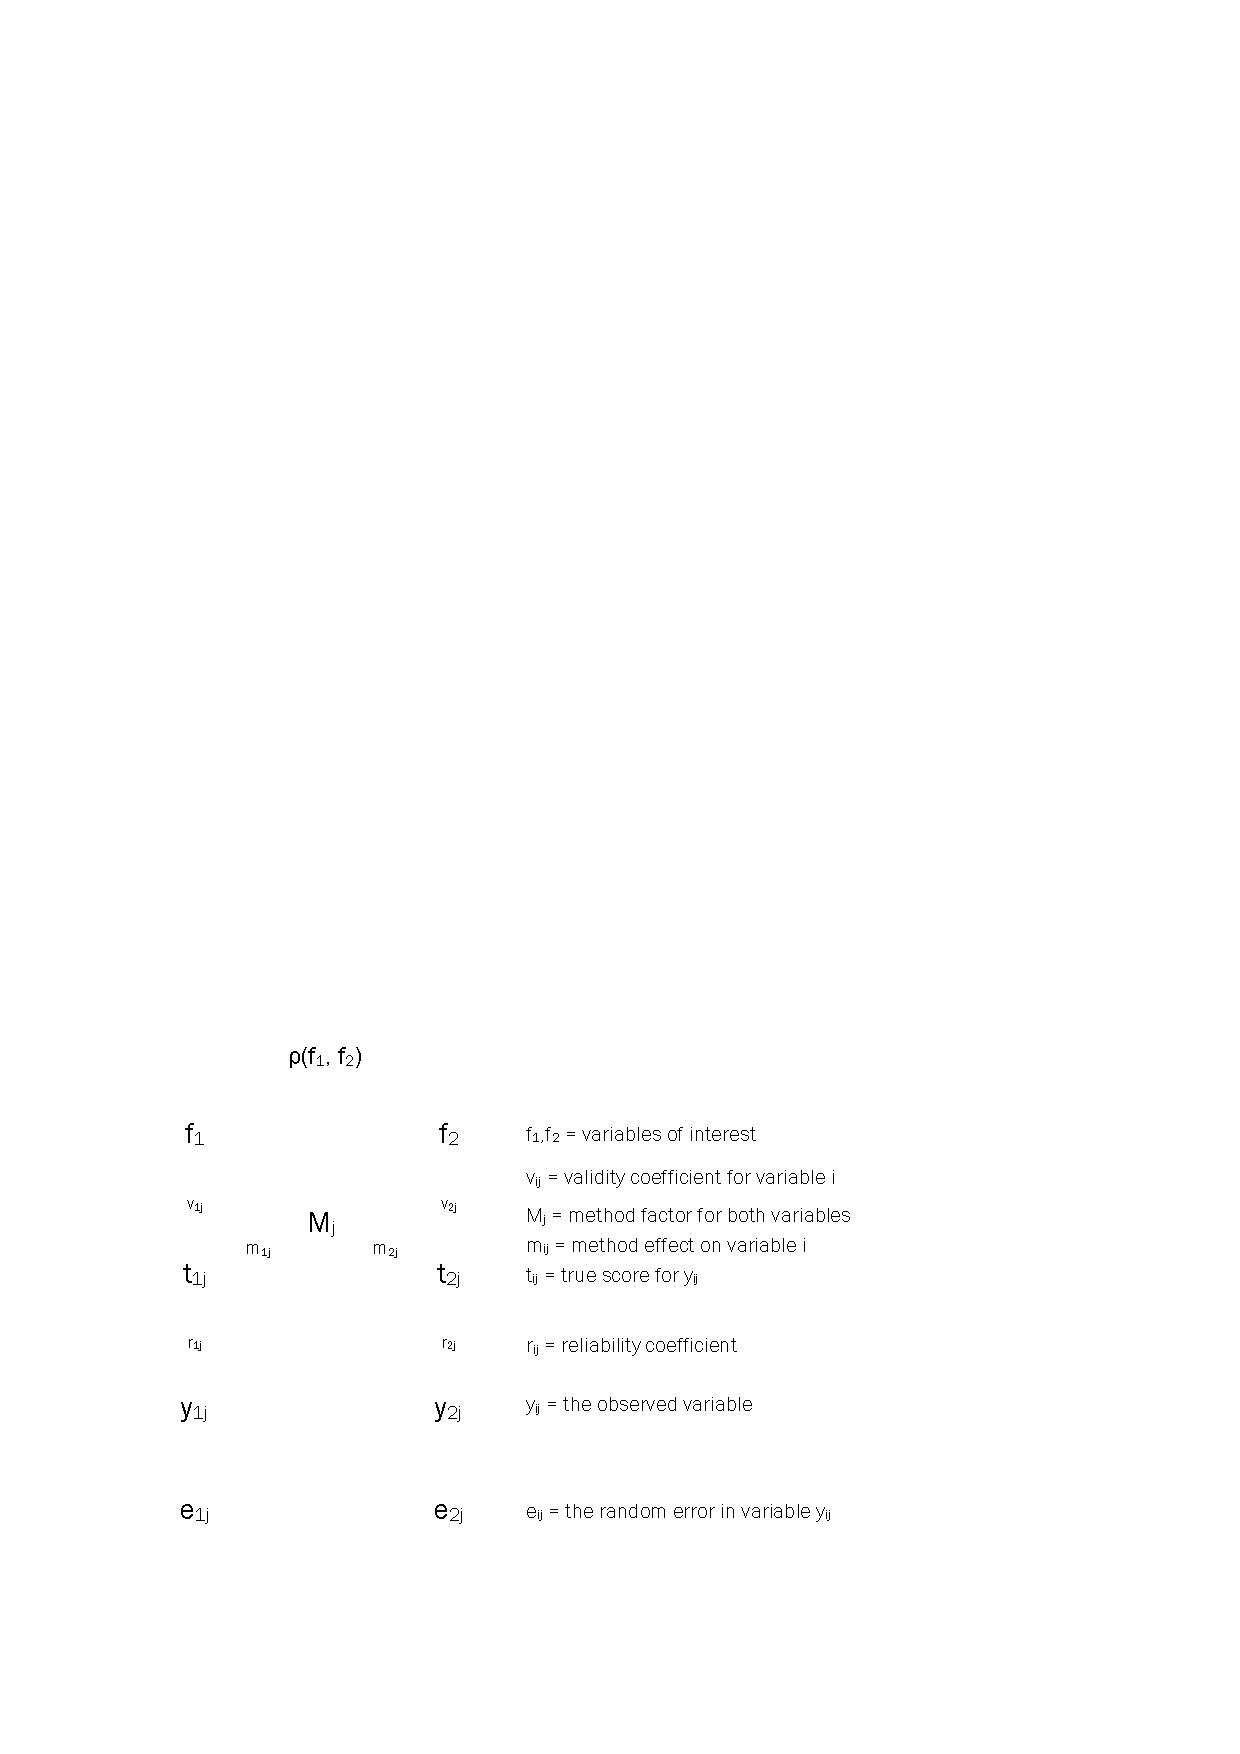
\includegraphics[height=7cm]{i/response-model.pdf}\\
\end{frame}

\begin{frame}	
	\frametitle{The basic response model}
	\begin{itemize}[<alert@+>]
		\item The quality coefficient $q$ is the product of the reliability and validity coefficients:
		\item $q = vr$
		\item The square $q^2$ is called the 'total quality' of a measure.
		\item It is the percentage of variance in the observed variable that can be explained by the latent variable of interest.
	\end{itemize}
\end{frame}	

\subsection{An example experiment}
\begin{frame}
	\frametitle{First trait measured with three methods}
	\begin{tabular}{l}
		\hline
		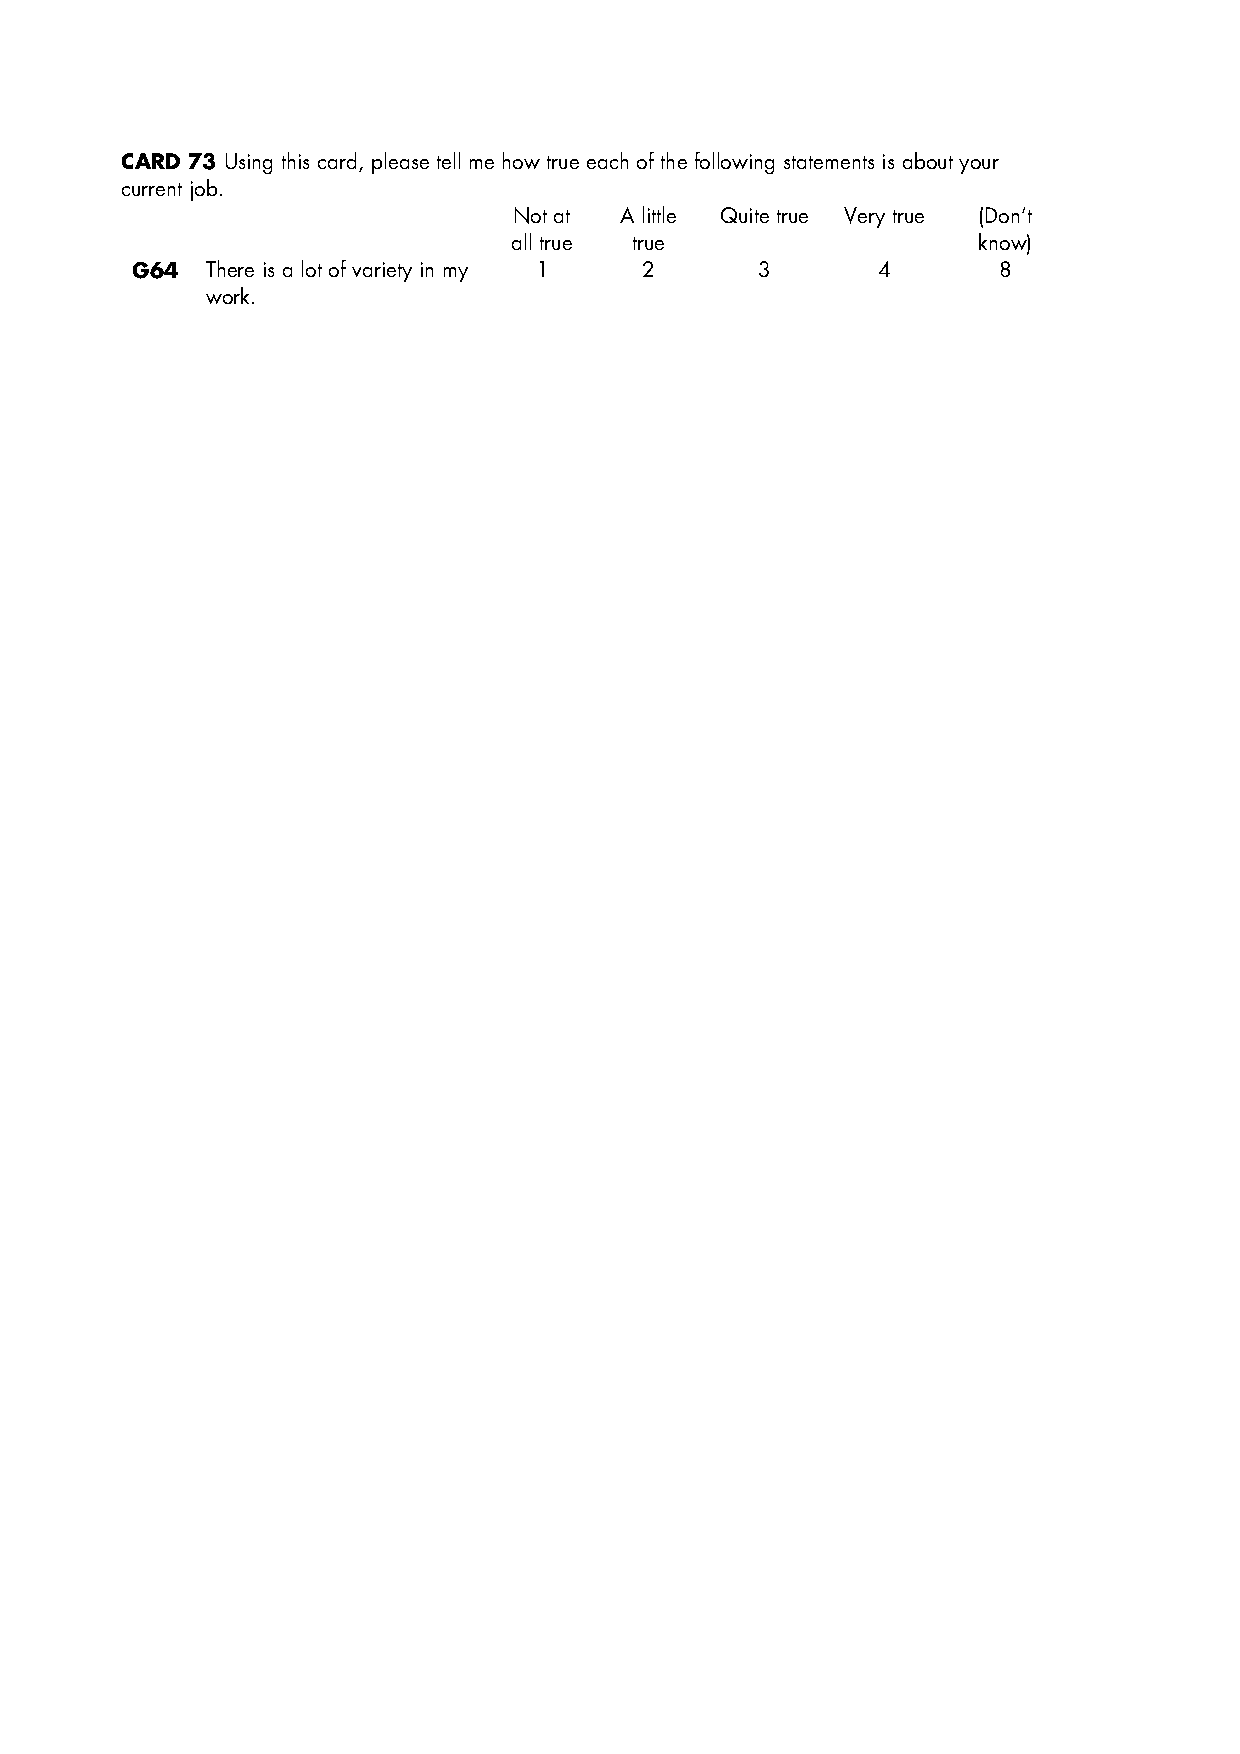
\includegraphics[width=8cm]{i/trait-1-m-1.pdf} \\\hline
		
\includegraphics[width=8cm]{i/trait-1-m-2.pdf} \\\hline
		 
\includegraphics[width=8cm]{i/trait-1-m-3.pdf}\\
		\hline
	\end{tabular}
\end{frame}

\begin{frame}
	\frametitle{Three traits measured with first method}
		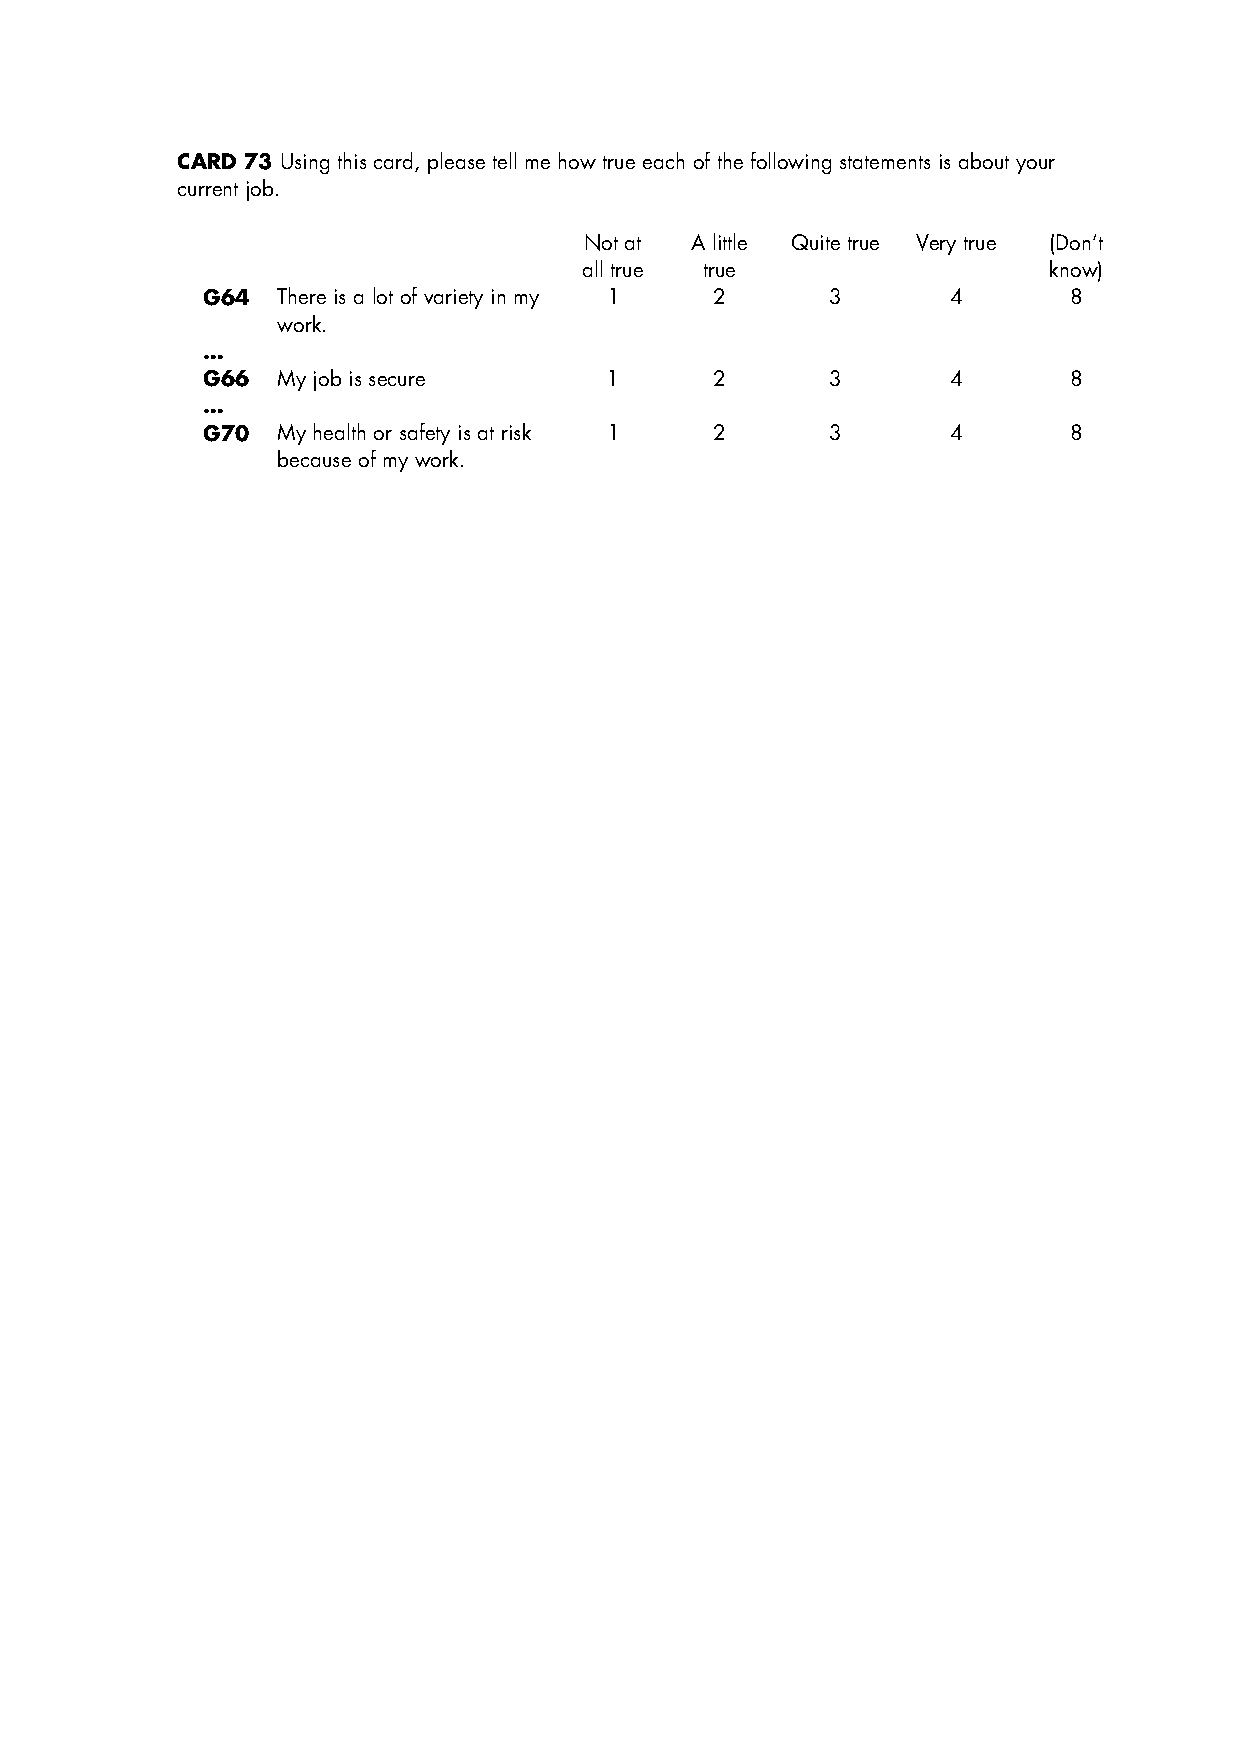
\includegraphics[width=11.2cm]{i/method-1.pdf}
\end{frame}

\begin{frame}
	\frametitle{Three traits measured with second method}
		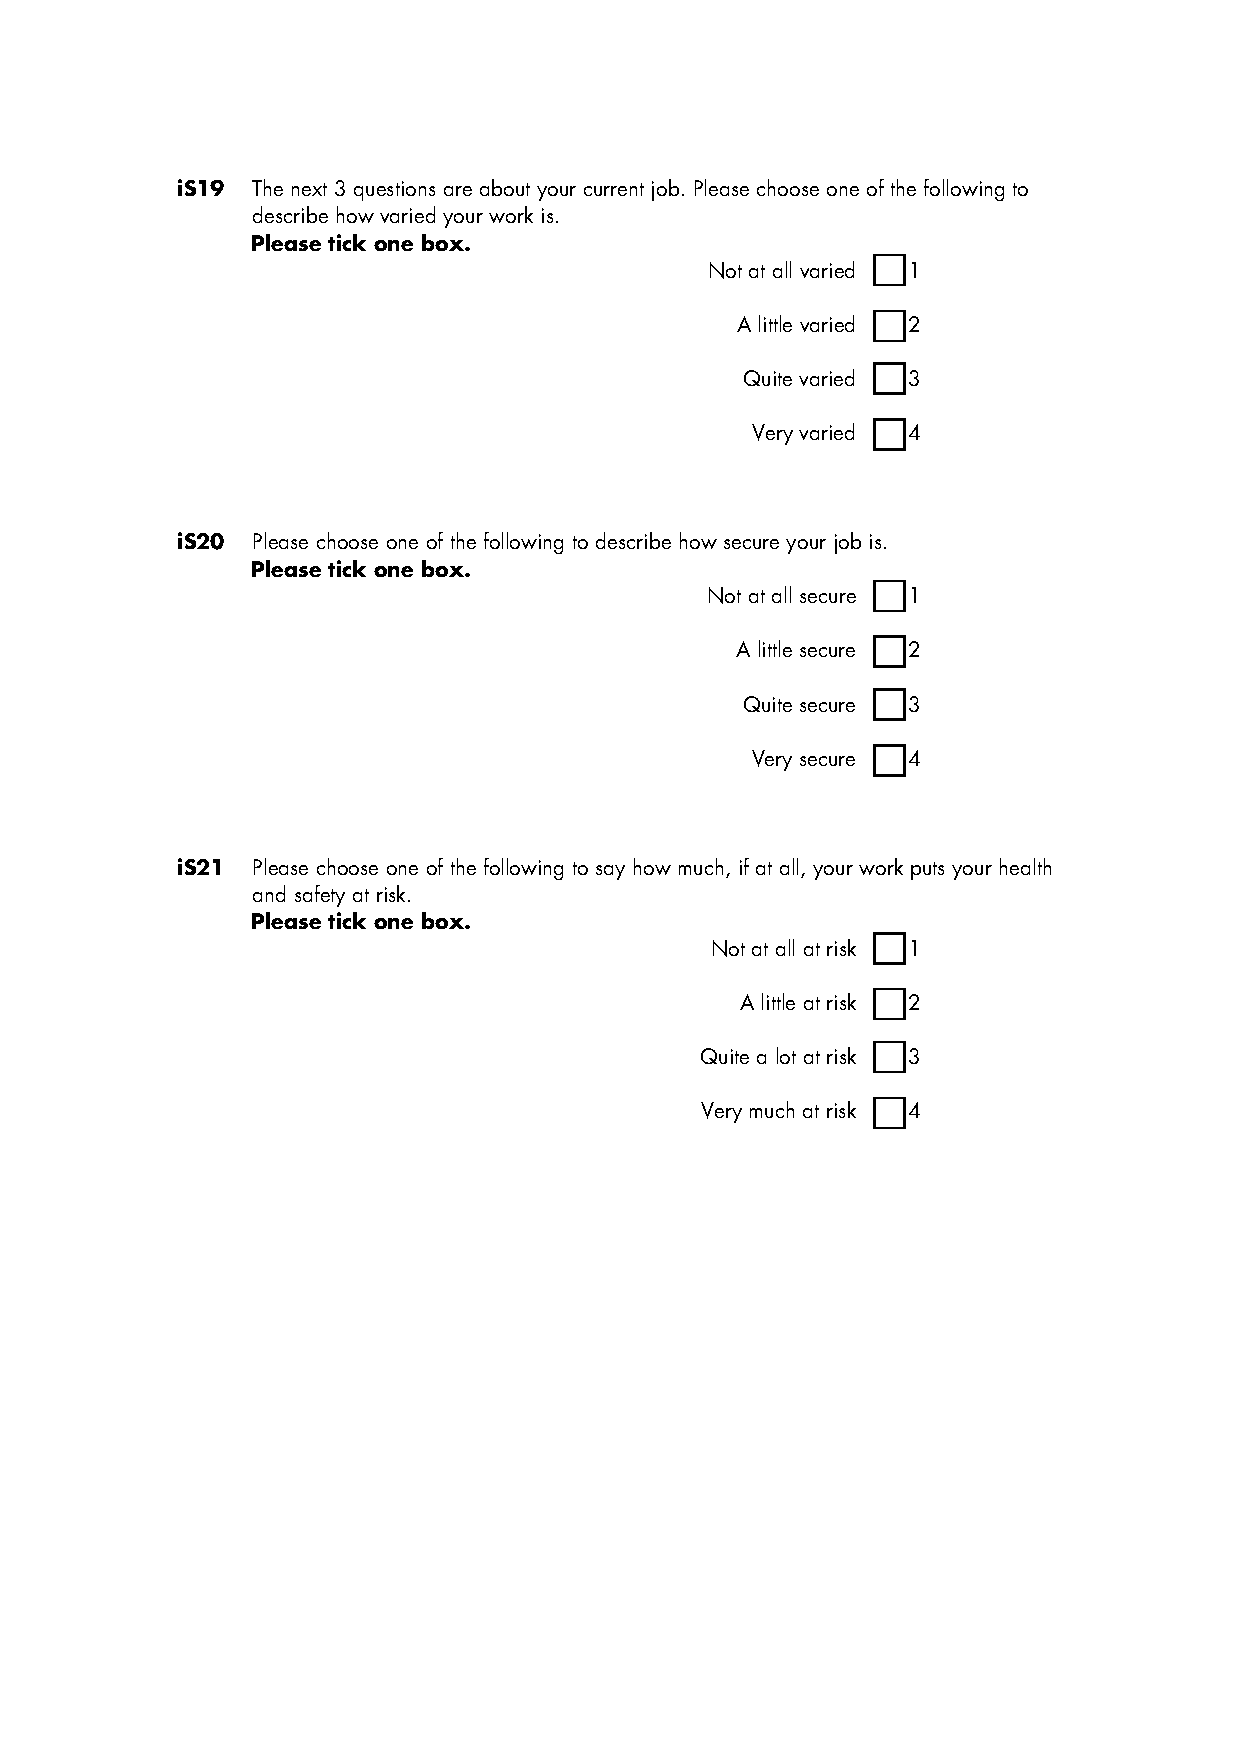
\includegraphics[height=7cm]{i/method-2.pdf}
\end{frame}

\begin{frame}
	\frametitle{Three traits measured with third method}
	\begin{columns}[T]
		\begin{column}{7cm}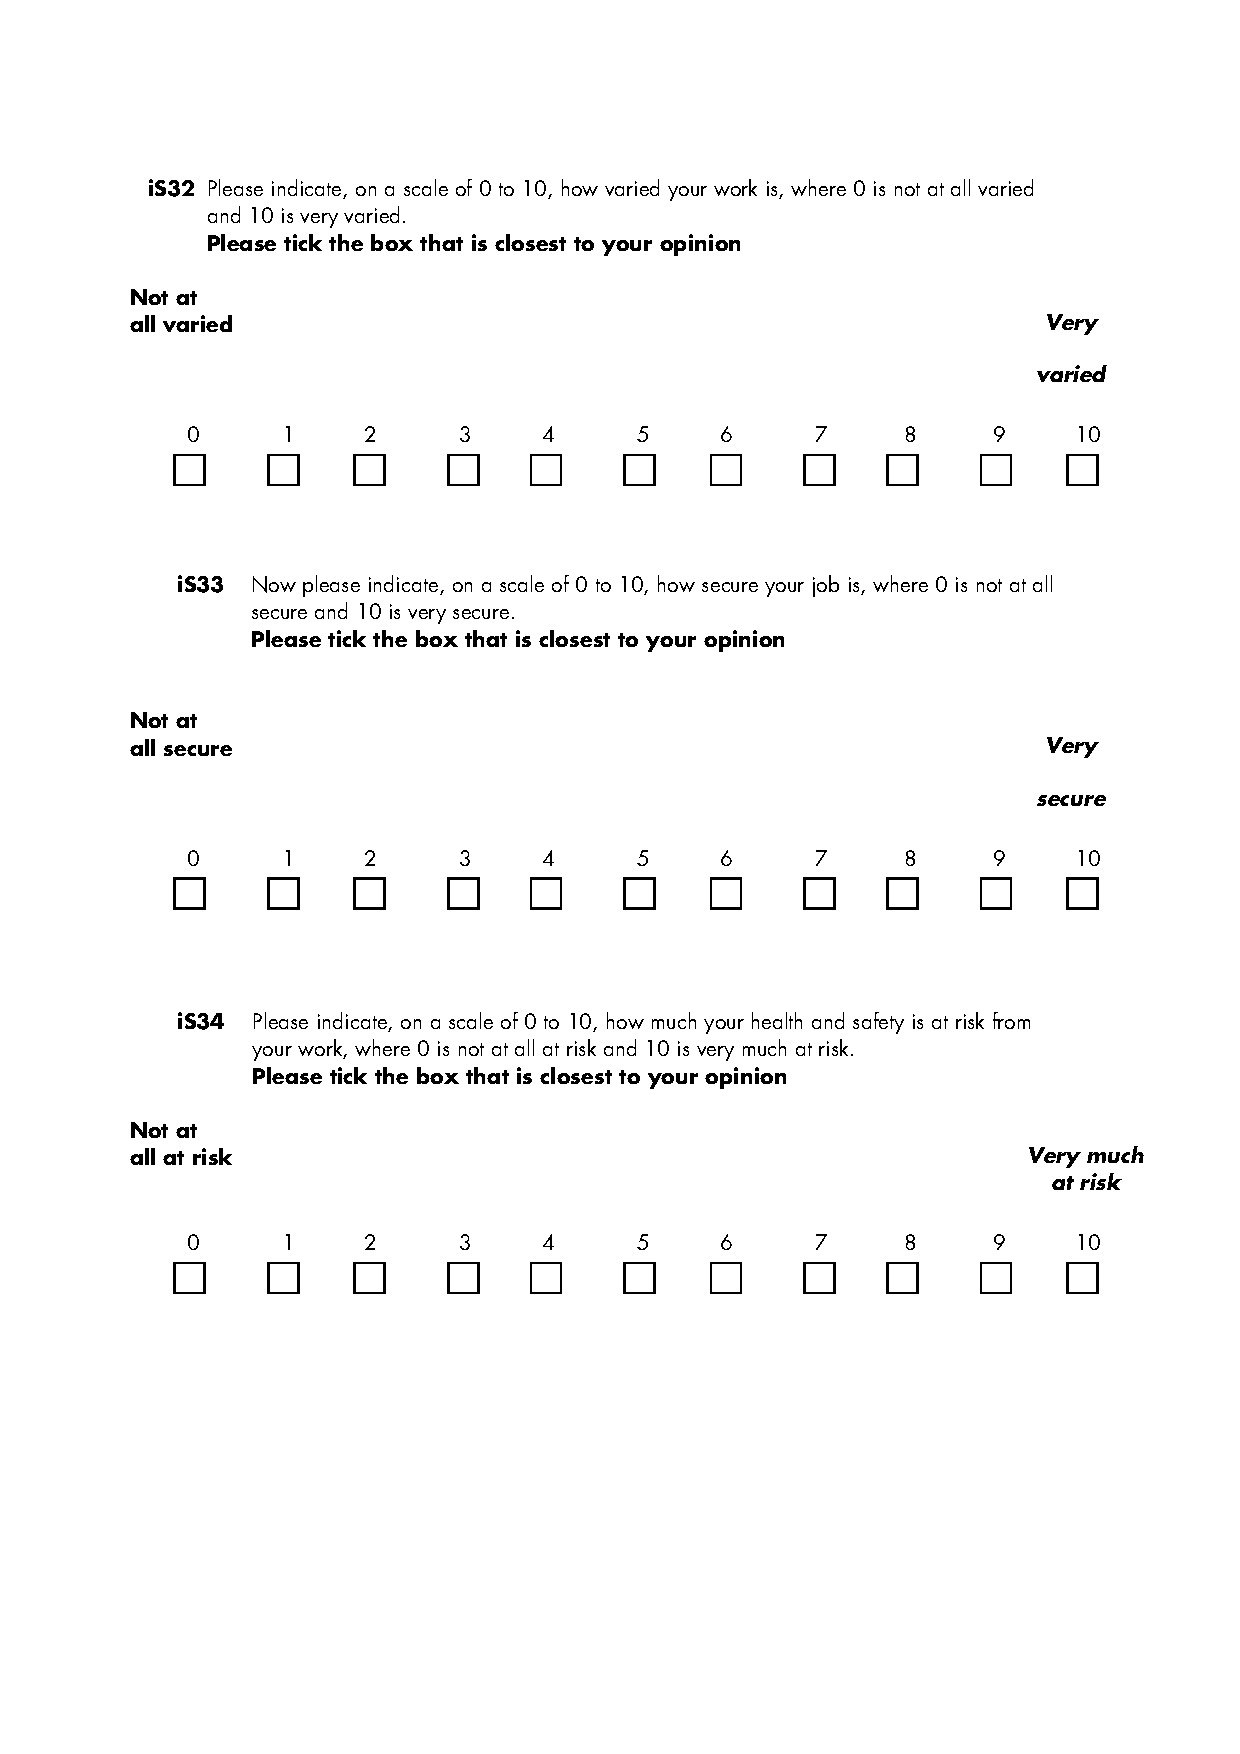
\includegraphics[height=7cm]{i/method-3.pdf}\end{column}
		\begin{column}{3cm}\hyperlink{model}{\beamerbutton{Skip details of the model}}\end{column}
	\end{columns}		
\end{frame}

\if 1=2
\subsection{Designs}

\begin{frame}	
	\frametitle{Split ballot design}

	\begin{itemize}[<alert@+>]
		\item Different designs are possible
		\item If 3 traits are asked using 3 methods, the respondent has to answer 
			$3 \times 3 = 9$ questions per experiment
		\item Answering the same question 3 times, for three different questions is a large response burden
		\item The solution: split ballot MTMM design.
\item<5-|alert@5> {
	Split the sample into groups A and B:

	\begin{tabular}{llccc}
\hline
		&&\multicolumn{3}{c}{Trait}\\
		& Method & 1 & 2 & 3\\
\hline
		Main quest. 	& 1 & A,B & A,B & A,B\\
		Supplementary quest.	& 2 & A & A & A\\
							& 3 & B & B & B\\
\hline
	\end{tabular}	}
	\end{itemize}

\end{frame}	
\fi

\subsection{Models}

\begin{frame}	
	\frametitle{Different models for MTMM experiments}
	\begin{itemize}[<alert@+>]
		\item Classic MTMM model
		\item Correlated uniqueness (Kenny \& Judd)
		\item Direct product (Browne)
		\item True score model
		\item MTM-1 (Eid 2000)
	\end{itemize}
\end{frame}	
\begin{frame}	
	\frametitle{Different models for MTMM experiments}
	\begin{itemize}[<alert@+>]
		\item We use the true score model
		\item Equivalent to the classic MTMM model
		\item Sometimes necessary to remove one method factor
		\item In that case our model is the equivalent to Eid's MTM-1 model.
	\end{itemize}
\end{frame}	

\begin{frame}	
	\frametitle{\hypertarget{model}{True score model}}
	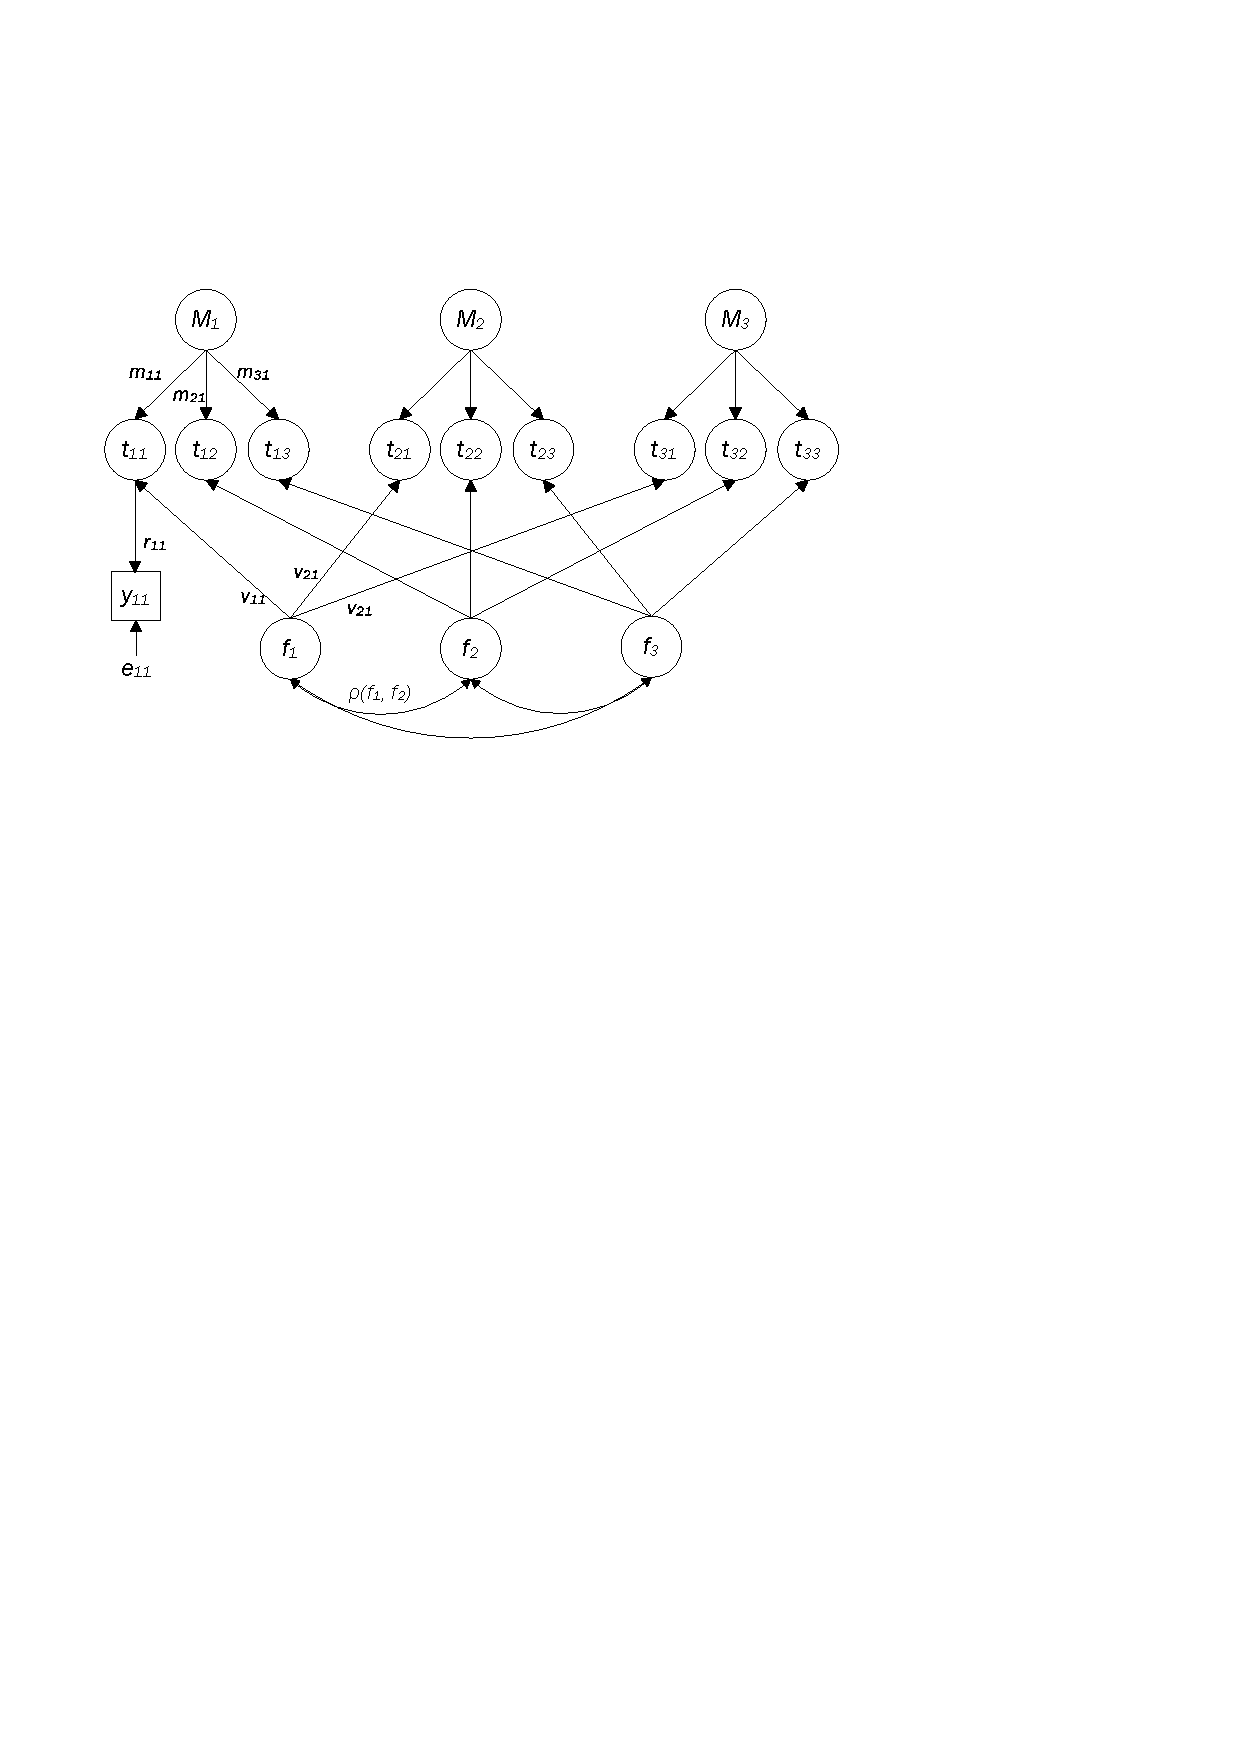
\includegraphics[height=7cm]{i/MTMM.pdf}
	\framezoom<1><2>(0cm,1.85cm)(.5cm,4.5cm)
	\framezoom<1><3>(0cm,0cm)(1cm,3cm)
\end{frame}	

\begin{frame}	
	\frametitle{True score model assumptions}
	\begin{itemize}[<alert@+>]
		\item No correlations among methods
		\item No correlations between traits and methods
		\item Equal method effects
		\item Linear and additive effects
		\item Normal errors, independent of all unobserved variables
		\item All variables are continuous
	\end{itemize}
\end{frame}	


\section{What has been done before}

\subsection{The international research project 1984--1996}


\begin{frame}
\frametitle{Countries in the international survey project 1984--1996\\that have been included in SQP}
	\begin{columns}[T]	
		\begin{column}{8cm}
			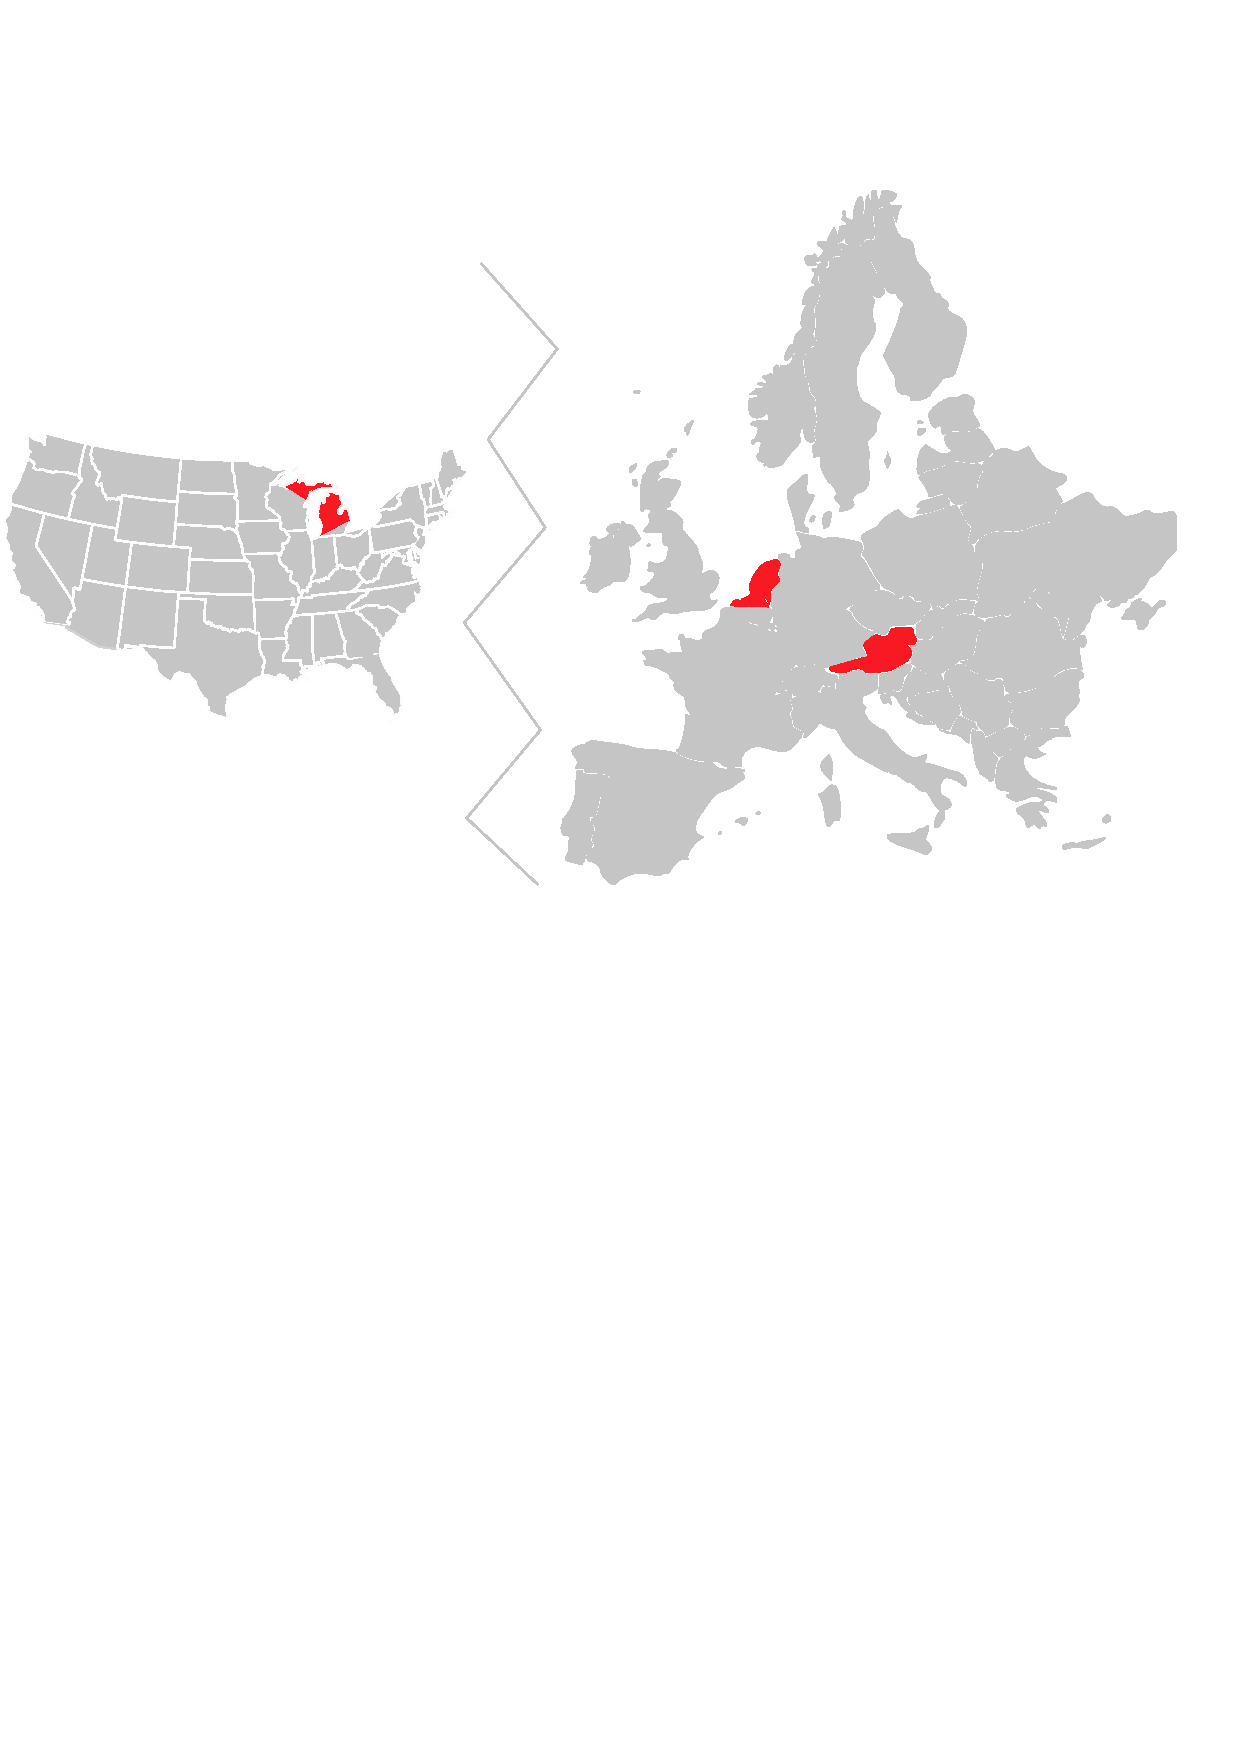
\includegraphics[width=\textwidth]{i/andrews-etal.pdf}
		\end{column}
		\begin{column}{3.2cm}
		\begin{small}
		\begin{enumerate}
			\item Austria 
			\item Belgium: Flanders
			\item Netherlands
			\item United States: Michigan		
		\end{enumerate}
		\end{small}
		\end{column}
	\end{columns}
\end{frame}

\subsection{Experiments in the European Social Survey}

\begin{frame}
	\frametitle{The European Social Survey (ESS)}

	
\includegraphics[width=2.8cm]{i/ess-logo.pdf}
	\begin{itemize}
		\item Three rounds, 4th coming up
		\item Six experiment in each round
		\item \texttt{http://www.europeansocialsurvey.org}
	\end{itemize}
\end{frame}

\begin{frame}

\frametitle{Countries in round 1 of the ESS -- 2002}

	\begin{columns}[T]	
		\begin{column}{5.5cm}
			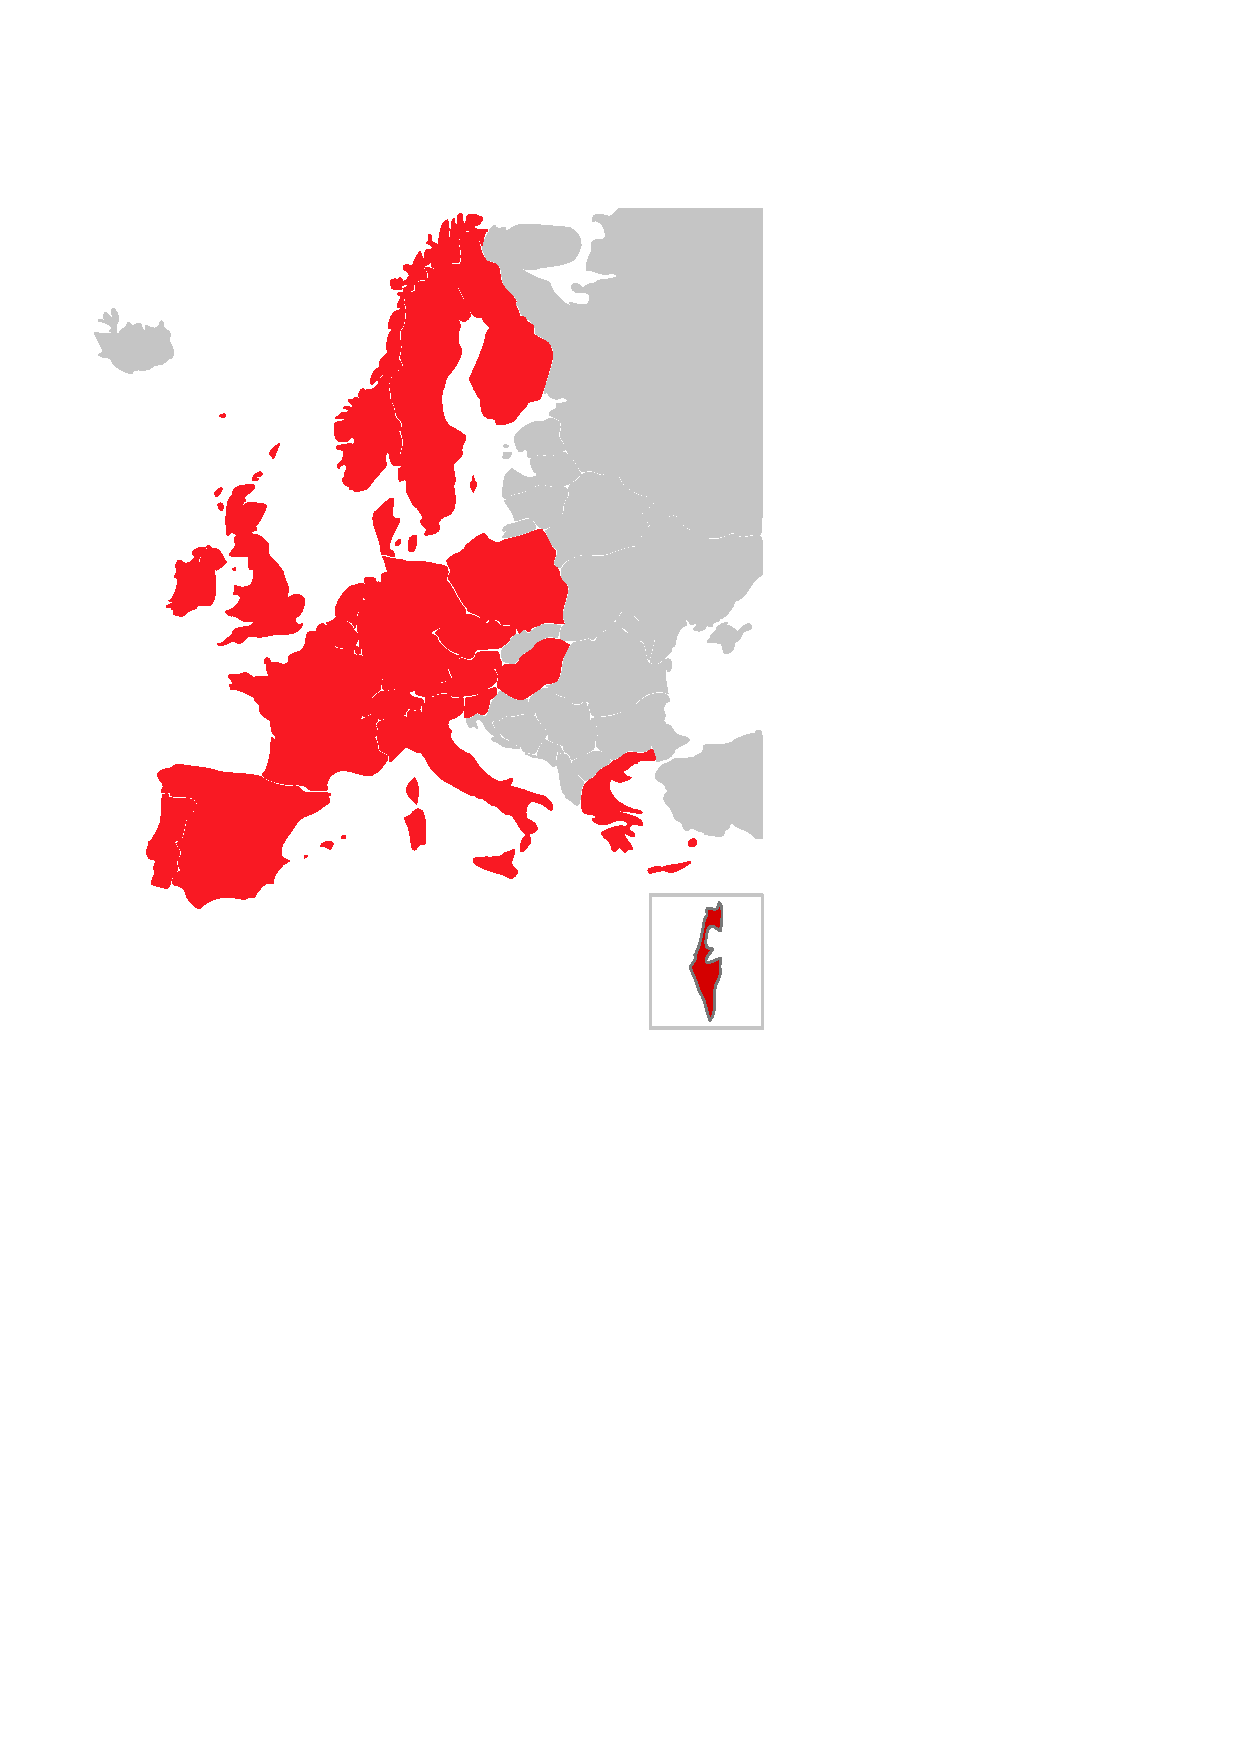
\includegraphics[width=\textwidth]{i/round1.pdf}
		\end{column}
		\begin{column}{4.5cm}
			\begin{columns}	
				\begin{column}{2.2cm}
					\begin{scriptsize}\begin{enumerate}
						\item Austria
						\item Belgium	
						\item Czech Republic 
						\item Denmark 	
						\item Finland 	
						\item France 	
						\item Germany 	
						\item Greece
						\item Hungary 
						\item Ireland 
						\item Israel 	
						\item Italy 										
					\end{enumerate}\end{scriptsize}
				\end{column}
				\begin{column}{2.5cm}
					\begin{scriptsize}\begin{enumerate}			
						\item[13.] Luxembourg			
						\item[14.] Netherlands
						\item[15.] Norway
						\item[16.] Poland
						\item[17.] Portugal
						\item[18.] Slovenia
						\item[19.] Spain
						\item[20.] Sweden
						\item[21.] Switzerland
						\item[22.] United Kingdom
					\end{enumerate}\end{scriptsize}
				\end{column}
			\end{columns}
		\end{column}
	\end{columns}
\end{frame} % to enforce entries in the table of contents

\begin{frame}

\frametitle{Countries in round 2 of the ESS -- 2004}

	\begin{columns}[T]	
		\begin{column}{6.5cm}
			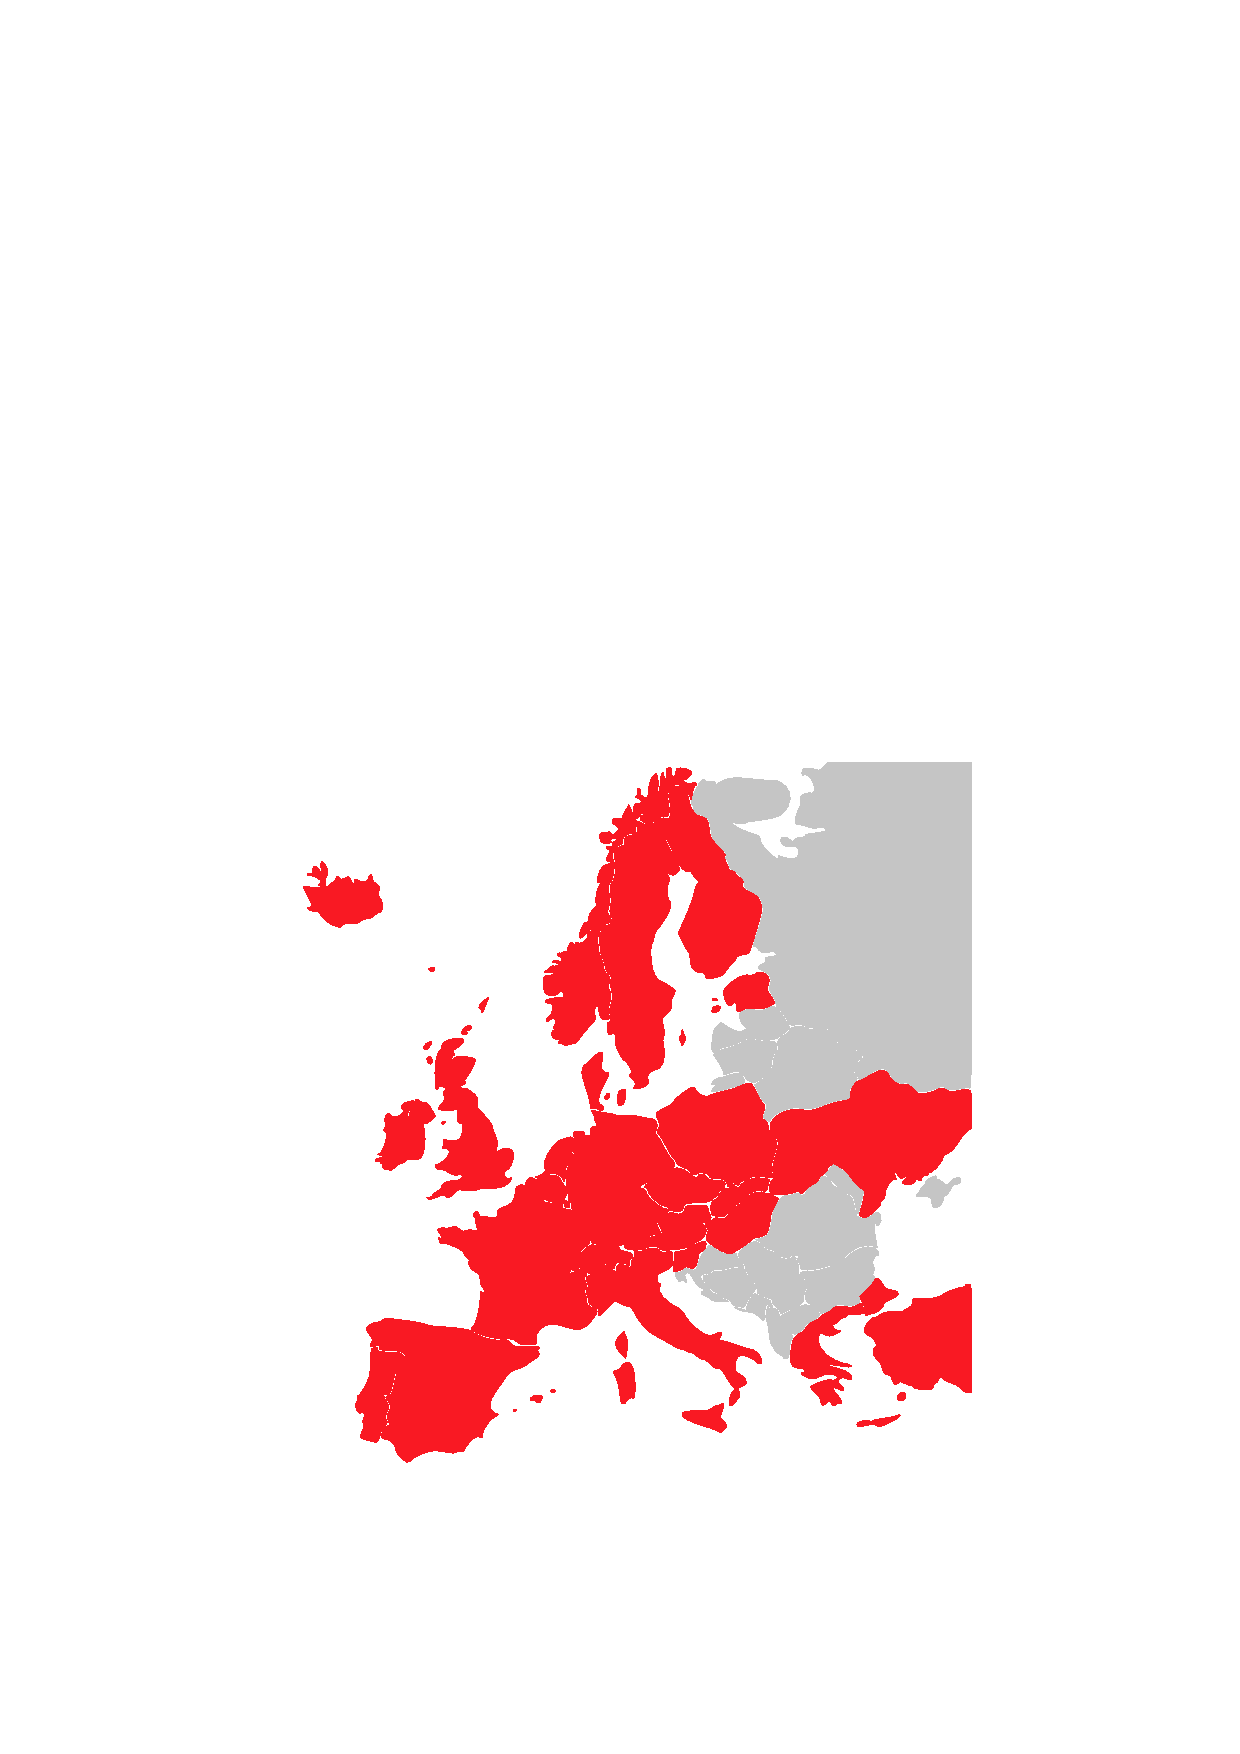
\includegraphics[width=\textwidth]{i/round2.pdf}
		\end{column}
		\begin{column}{4.5cm}
			\begin{columns}	
				\begin{column}{2cm}
					\begin{scriptsize}\begin{enumerate}
            \item Austria 	        
						\item Belgium 	        
						\item Czech Republic 	
						\item Denmark 	        
						\item Estonia 	        
						\item Finland 	        
						\item France 	        
						\item Germany 	        
						\item Greece 	        
						\item Hungary 	        
						\item Iceland 	        
						\item Ireland 	        		
            \item Italy 	
        \end{enumerate}\end{scriptsize}
				\end{column}
				\begin{column}{2.5cm}
					\begin{scriptsize}\begin{enumerate}			
						\item[14.] Luxembourg 	
						\item[15.] Netherlands 	
						\item[16.] Norway 	
						\item[17.] Poland 	
						\item[18.] Portugal 	
						\item[19.] Slovakia 	
						\item[20.] Slovenia 	
						\item[21.] Spain 	
						\item[22.] Sweden 	
						\item[23.] Switzerland 	
						\item[24.] Turkey 	
						\item[25.] Ukraine 	
						\item[26.] United Kingdom 						
\end{enumerate}\end{scriptsize}
				\end{column}
			\end{columns}
		\end{column}
	\end{columns}
\end{frame}

\begin{frame}

\frametitle{Countries in round 3 of the ESS -- 2006}

	\begin{columns}[T]	
		\begin{column}{6.5cm}
			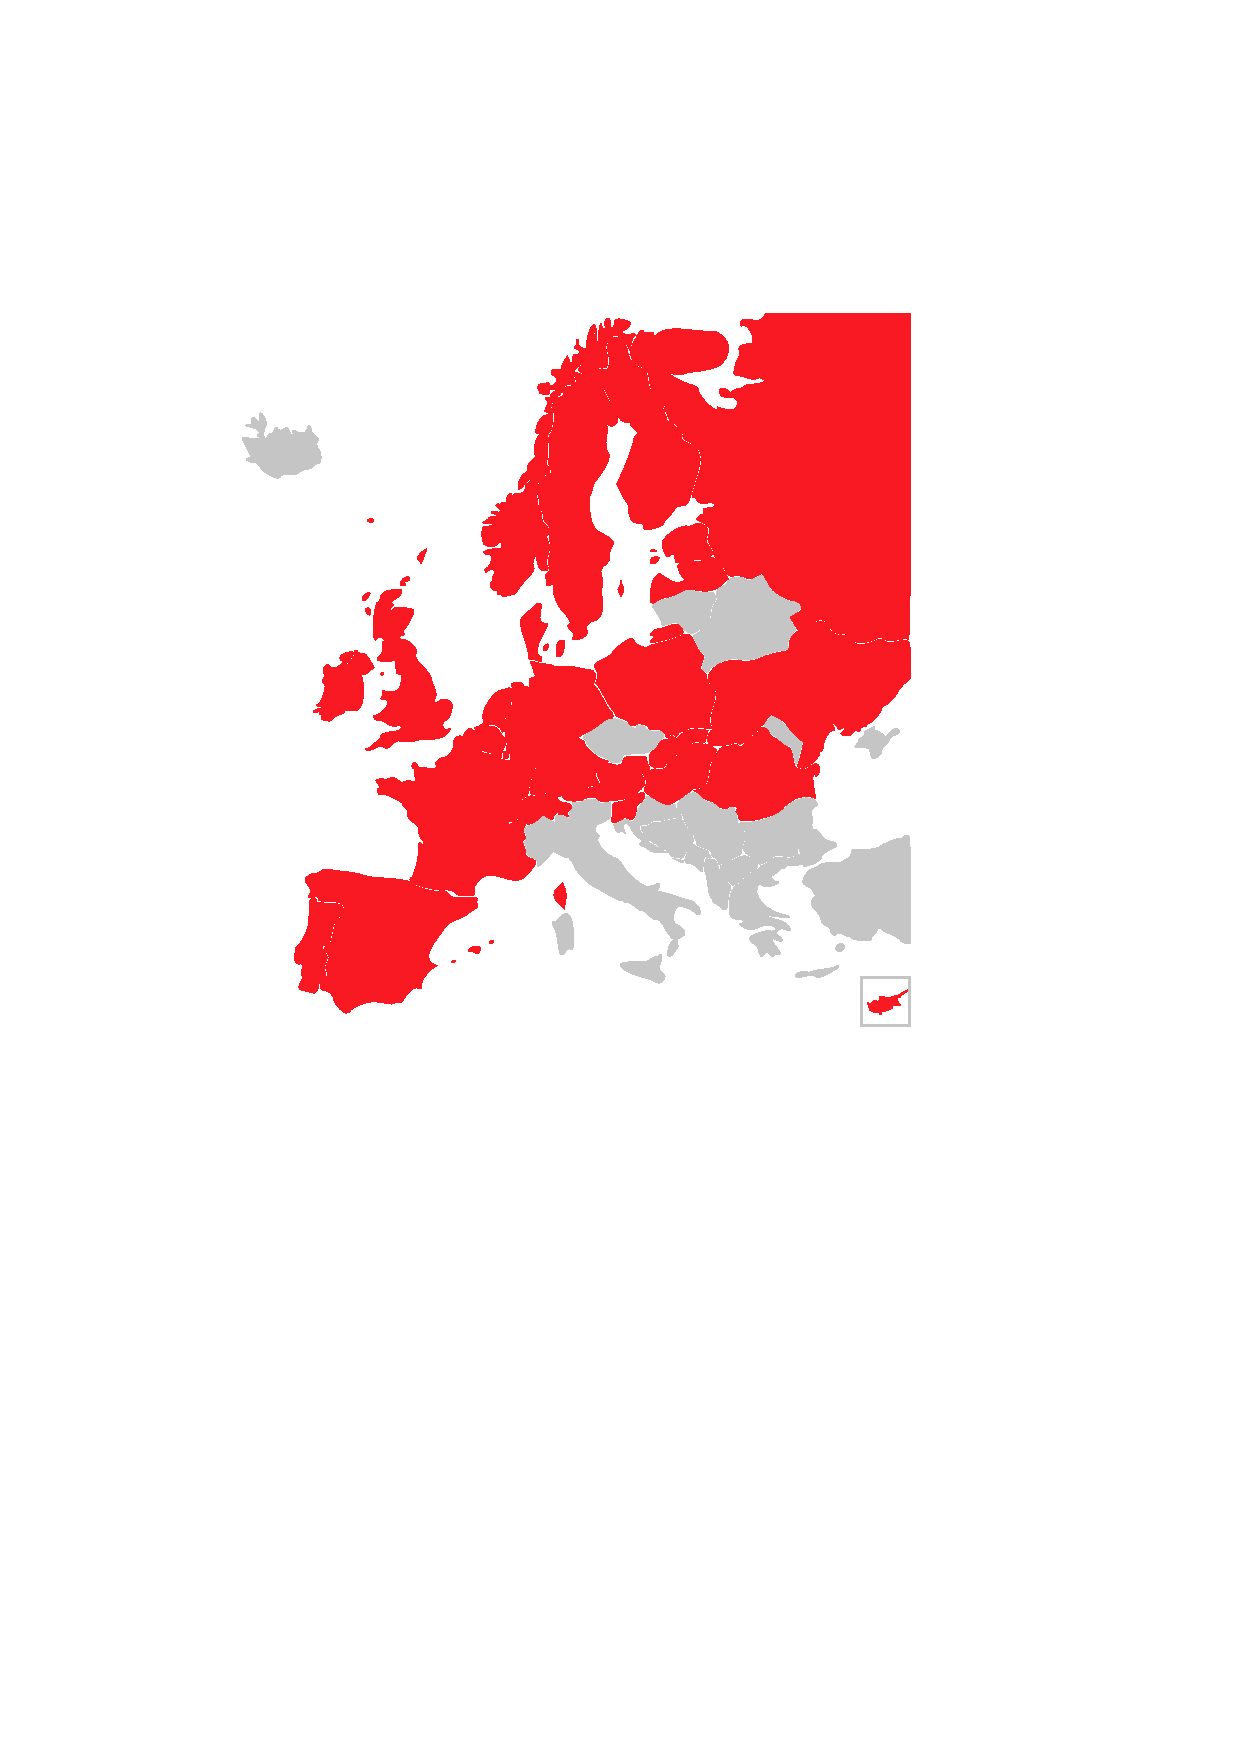
\includegraphics[width=\textwidth]{i/round3.pdf}
		\end{column}
		\begin{column}{4.5cm}
			\begin{columns}	
				\begin{column}{2cm}
					\begin{scriptsize}\begin{enumerate}
						\item Austria
						\item Belgium 	
						\item Bulgaria 	
						\item Cyprus 	
						\item Denmark 	
						\item Estonia 	
						\item Finland 	
						\item France 	
						\item Germany 	
						\item Hungary 	
						\item Ireland
						\item Latvia													
					\end{enumerate}\end{scriptsize}
				\end{column}
				\begin{column}{2.5cm}
					\begin{scriptsize}\begin{enumerate}		
						\item[13.] Netherlands			
						\item[14.] Norway 	
						\item[15.] Poland 	
						\item[16.] Portugal 	
						\item[17.] Romania 	
						\item[18.] Russian Federation 	
						\item[19.] Slovakia 	
						\item[20.] Slovenia 	
						\item[21.] Spain 	
						\item[22.] Sweden 	
						\item[23.] Switzerland 	
						\item[24.] Ukraine
						\item[25.] United Kingdom 
					\end{enumerate}\end{scriptsize}
				\end{column}
			\end{columns}
		\end{column}
	\end{columns}
\end{frame}
% topics

\begin{frame}
\frametitle{Some results from rounds 1 and 2}
\begin{table}[hbt]\centering\begin{footnotesize}
\begin{tabular}{lrrrr}
\hline
Country&Mean&Median&Minimum&Maximum\\\hline
Portugal&0.79&0.81&0.63&0.91\\
Switzerland&0.79&0.84&0.56&0.90\\
Greece&0.78&0.79&0.64&0.90\\
Estonia&0.78&0.85&0.58&0.90\\
Poland&0.73&0.85&0.51&0.90\\
Luxembourg&0.72&0.73&0.53&0.88\\
United Kingdom&0.70&0.71&0.56&0.82\\
Denmark&0.70&0.70&0.52&0.80\\
Belgium&0.70&0.73&0.46&0.90\\
Germany&0.69&0.70&0.53&0.83\\
Spain&0.69&0.64&0.54&0.90\\
Austria&0.68&0.68&0.51&0.85\\
Czech Republic&0.65&0.60&0.52&0.87\\
Slovenia&0.63&0.60&0.46&0.82\\
Norway&0.59&0.59&0.35&0.83\\
Sweden&0.58&0.58&0.43&0.68\\
Finland&0.57&0.54&0.42&0.78\\
	\hline
\end{tabular}\end{footnotesize}
\end{table}
\end{frame}

\section{Why are there differences between countries?}

\begin{frame}
\frametitle{Differences between countries?}

What we studied already:

\begin{itemize}[<alert@+>]
	\item Differences in complexity of language? 
		\begin{itemize}[<2-|alert@+>]\item{Not found}\end{itemize}
	\item Artifacts due to sending in the questionnaire later?
		\begin{itemize}[<4-|alert@+>]\item{Only Sweden, Norway, Finland}\end{itemize} 
	\item Artifacts due to mistakes in translation?
		\begin{itemize}[<6-|alert@+>]\item{Two cases found for two experiments}\end{itemize} 
	\item<7-|alert@+> None of these findings suffice to explain the large differences we found!
	\item<8-|alert@+> Differences in use of the scale?
\end{itemize}

\end{frame}

\begin{frame}
	\frametitle{Categorisation of continuous variables}

    Our model assumes that there are \emph{unobserved} continuous latent response variables (LRV) that have been categorised into the \emph{observed} categorical variables.

 \begin{columns}<2->[T]
 	\begin{column}{4.5cm}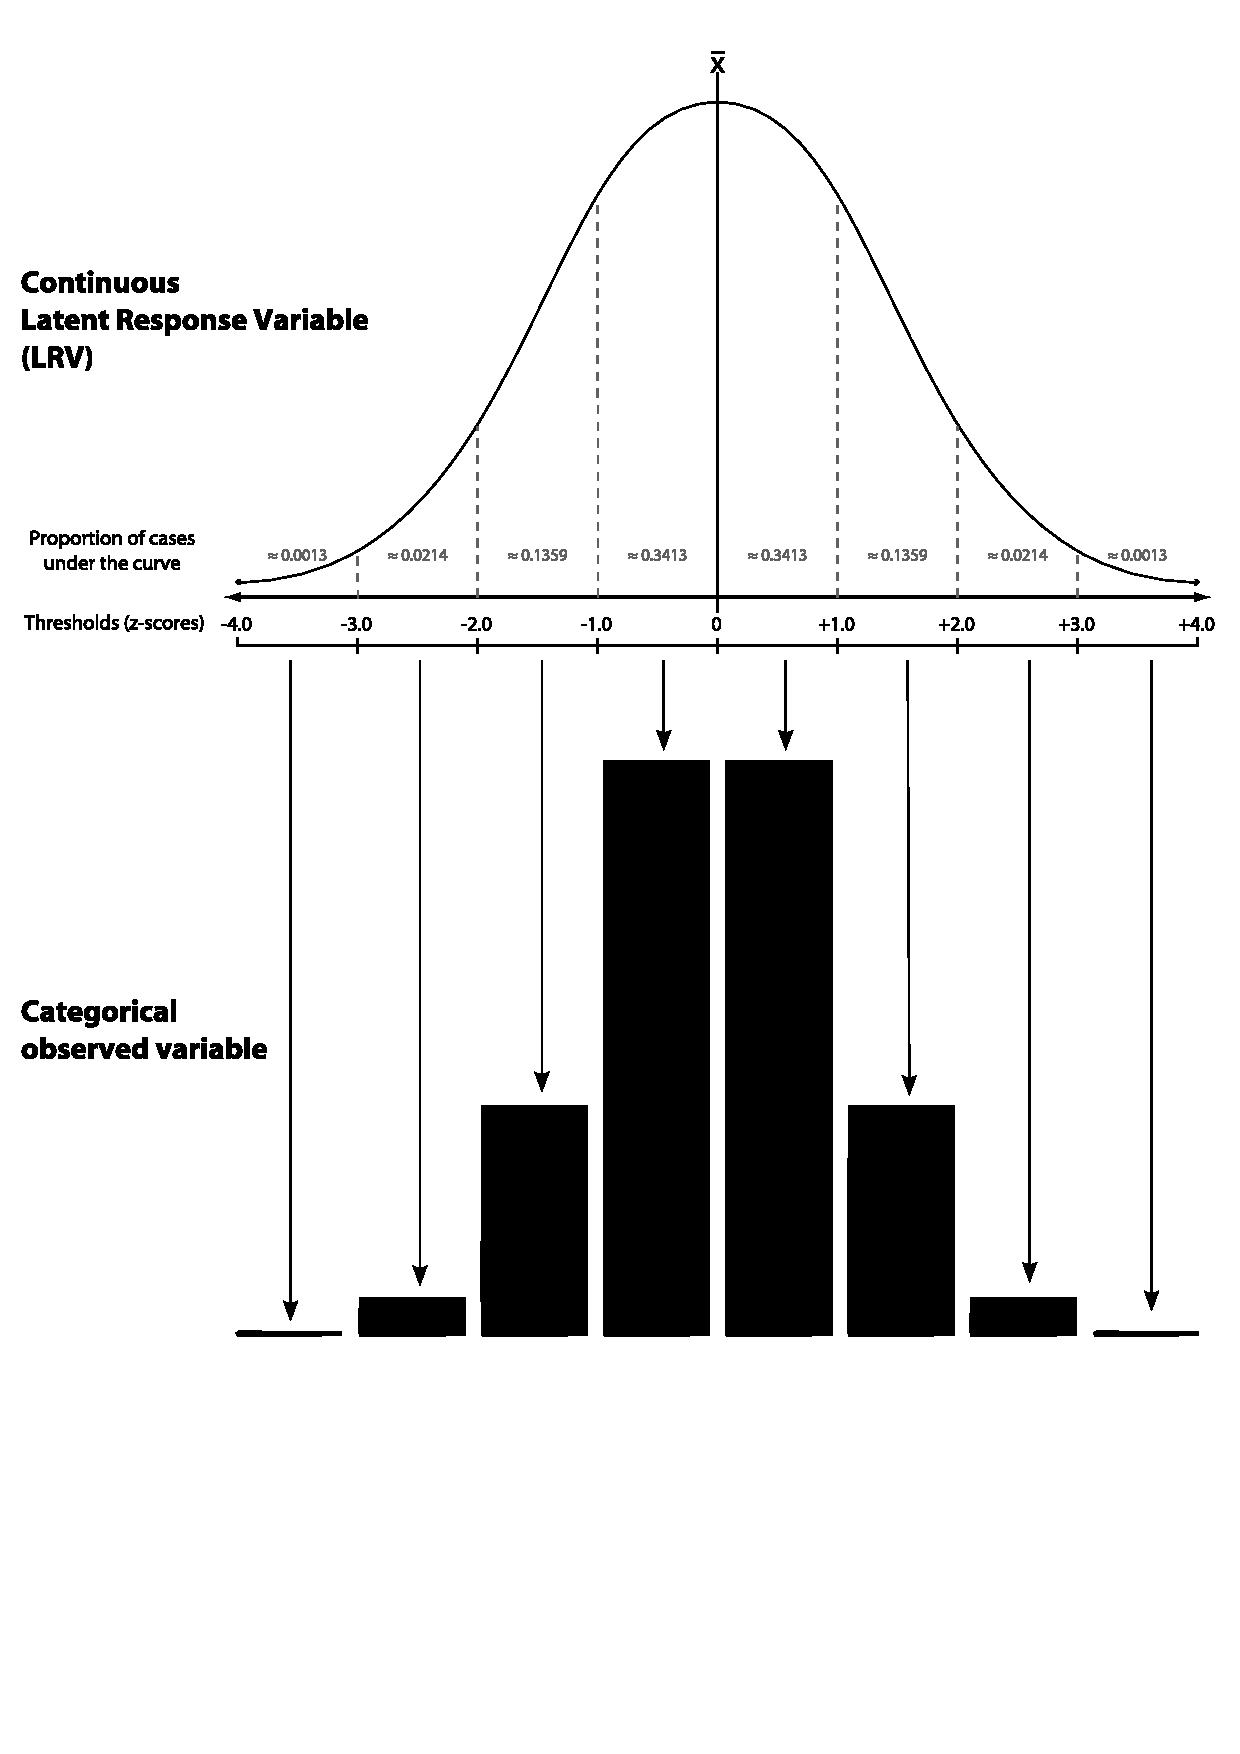
\includegraphics[width=4.5cm]{i/LRV-8cat.pdf}\end{column}
 	\begin{column}<3->{4.5cm}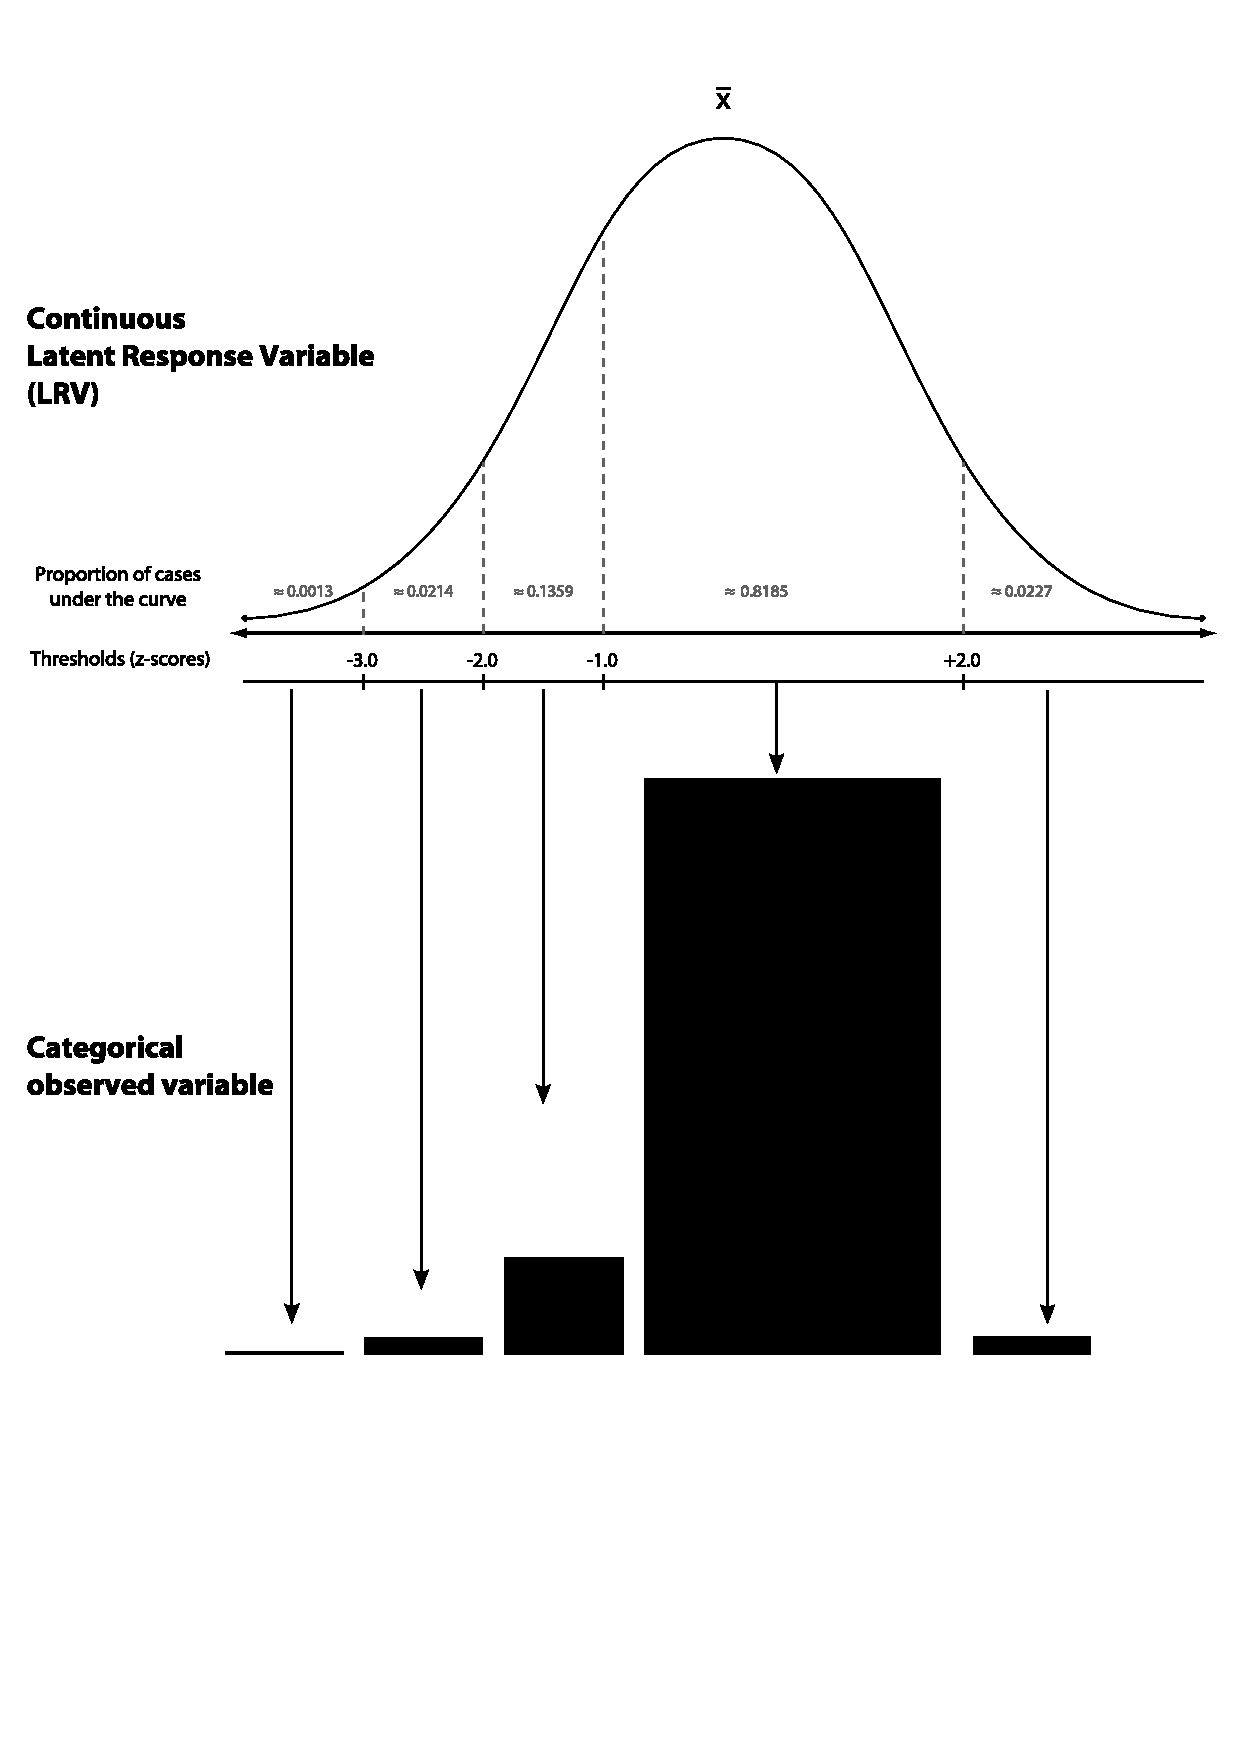
\includegraphics[width=4.5cm]{i/LRV-skew.pdf}
 	\end{column}
 \end{columns}
\end{frame}

\begin{frame}
    \begin{itemize}
    \item These continuous latent response variables are related to each other according to the MTMM model.
	\item Method effects, quality coefficients, and thresholds can be estimated.
    \item Equivalent to a 2 parameter graded response model in IRT (Muth\'en \& Asparouhov 2002).
	\item We call the ratio of the quality coefficient $q = v.r$ from the categorical model to the same coefficient from the continuous model the `categorisation factor'.
    \end{itemize}
\end{frame}


\begin{frame}
\frametitle{Consequences of categorisation for the correlations between observed variables}

	\begin{itemize}[<alert@+>]
		\item The fewer categories, the smaller the Pearson correlation
		\item The more skew in observed variables, the smaller the Pearson correlation
		\item The corrected (`polychoric') correlations are always higher than the Pearson correlations, but not necessarily equally so for all variables.
	\end{itemize}
\end{frame}

\begin{frame} 
	Therefore,
	\begin{itemize}[<alert@+>]
		\item If the skewness of observed variables is higher for variables measured by one particular method, then the corrected correlations between those variables will go up more than the others, and the method effects in the categorical model will be higher.
		\item Higher estimated method effects can lower the estimate of quality in the categorical model.
		\item If this differs across countries, the process can possibly explain differences in the quality.
	\end{itemize} 
\end{frame}

\begin{frame}
\frametitle{Analysis of the experiments}

	\begin{itemize}[<alert@+>]
		\item We analysed the 4 experiments from the ESS which involved variables with 5 categories or less
		\item The topics: role of women, GP's, political efficacy, job.

			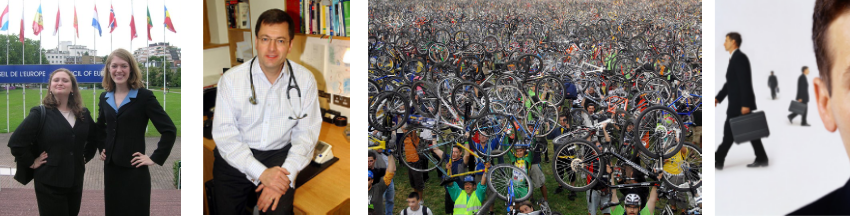
\includegraphics[width=10cm]{i/topics.png} 

	\item Compare the country with the highest quality to the country with the lowest quality for that experiment
	\end{itemize}


\end{frame}


\subsection{Categorisation errors in the efficacy experiment}

\begin{frame}
\frametitle{Quality ($q^2$)and method effects ($m$) in the efficacy experiment}

Continuous MTMM model, main questionnaire (first method)

\begin{footnotesize}\begin{tabular}{lllrrr}
\hline
 &  &  &  & `Efficacy' & \\
	   &  &  & Complex & Active & Mind\\
	   \hline
 &  $q^2$& Denmark & 0.77 & 0.83 & 0.79\\
 &  & Switzerland & 0.49 & 0.81 & 0.50\\
 &  $m$& Denmark & 0.00 & 0.00 & 0.00\\
 &  & Switzerland & 0.00 & 0.00 & 0.00\\
\hline
\end{tabular}\end{footnotesize}
\end{frame}


\begin{frame}
\frametitle{Efficacy experiment: Denmark}

Polychoric correlations

\begin{footnotesize}
\begin{tabular}{llrrrrrr}
 \hline
 &&\multicolumn{3}{c}{Method 1} & \multicolumn{3}{c}{Method 2}\\
 &&\multicolumn{3}{c}{$\overbrace{\hspace{90pt}}$} & \multicolumn{3}{c}{$\overbrace{\hspace{90pt}}$}\\
Method 1	& Complex 	& 1.00 &  &  &  &  & \\
			& Active 	& -0.44 & 1.00 &  &  &  & \\
			& Mind 		& -0.51 & 0.47 & 1.00 &  &  & \\
Method 2	& Complex 	& 0.66 & -0.45 & -0.51 & 1.00 &  & \\
			& Active 	& -0.44 & 0.74 & 0.46 & -0.51 & 1.00 & \\
			& Mind 		& -0.52 & 0.51 & 0.67 & -0.56 & 0.56 & 1.00\\
 \hline
 \end{tabular} 
 \end{footnotesize}

Pearson correlations

\begin{footnotesize}\begin{tabular}{llrrrrrr}
 \hline
 &&\multicolumn{3}{c}{Method 1} & \multicolumn{3}{c}{Method 2}\\

 &&\multicolumn{3}{c}{$\overbrace{\hspace{90pt}}$} & \multicolumn{3}{c}{$\overbrace{\hspace{90pt}}$}\\
Method 1	& Complex 	&  1.00 &  &  &  &  & \\
			& Active 	& -0.40 & 1.00 &  &  &  & \\
			& Mind 		& -0.47 & 0.37 & 1.00 &  &  & \\
Method 2	& Complex 	&  0.60 & -0.37 & -0.44 & 1.00 &  & \\
			& Active 	& -0.39 & 0.67 & 0.40 & -0.43 & 1.00 & \\
			& Mind 		& -0.46 & 0.43 & 0.62 & -0.49 & 0.48 & 1.00\\
 \hline
 \end{tabular} \end{footnotesize}
\end{frame}



\begin{frame}
\frametitle{Efficacy experiment: Switzerland}

Polychoric correlations

\begin{footnotesize}
\begin{tabular}{llrrrrrr}
 \hline
 &&\multicolumn{3}{c}{Method 1} & \multicolumn{3}{c}{Method 2}\\
 &&\multicolumn{3}{c}{$\overbrace{\hspace{90pt}}$} & \multicolumn{3}{c}{$\overbrace{\hspace{90pt}}$}\\
Method 1	& Complex 	& 1.00 & \\
			& Active 	& -0.37 & 1.00 & \\
			& Mind 		& -0.46 & 0.42 & 1.00 & \\
Method 2	& Complex 	& 0.57 & -0.36 & -0.46 & 1.00 & \\
			& Active 	& -0.32 & 0.83 & 0.36 & -0.39 & 1.00 & \\
			& Mind 		& -0.36 & 0.44 & 0.69 & -0.49 & 0.43 & 1.00\\
 \hline
 \end{tabular} 
 \end{footnotesize}

Pearson correlations

\begin{footnotesize}\begin{tabular}{llrrrrrr}
 \hline
 &&\multicolumn{3}{c}{Method 1} & \multicolumn{3}{c}{Method 2}\\

 &&\multicolumn{3}{c}{$\overbrace{\hspace{90pt}}$} & \multicolumn{3}{c}{$\overbrace{\hspace{90pt}}$}\\
Method 1	& Complex 	& 1.00 & \\
			& Active 	& -0.33 & 1.00 & \\
			& Mind 		& -0.34 & 0.36 & 1.00 & \\
Method 2	& Complex 	& 0.55 & -0.35 & -0.45 & 1.00 & \\
			& Active 	& -0.30 & 0.82 & 0.33 & -0.34 & 1.00 & \\
			& Mind 		& -0.35 & 0.41 & 0.62 & -0.48 & 0.39 & 1.00\\
 \hline
 \end{tabular} \end{footnotesize}
\end{frame}

\begin{frame}
\frametitle{\% Increase in the correlations after correction for categorisation}

Efficacy experiment: Denmark

\begin{tabular}{llrrrrrr}
\hline
 &&\multicolumn{3}{c}{Method 1} & \multicolumn{2}{c}{Method 2}  \\
&&\multicolumn{3}{c}{$\overbrace{\hspace{90pt}}$} & \multicolumn{3}{c}{$\overbrace{\hspace{60pt}}$}\\
 Method 1	& Complex 	& &  &  &  &  & \\
 			& Active 	& \textbf{8}\% &  &  &  & \\
 			& Mind 		& \textbf{8}\% & \textbf{29}\% &  &  & \\
 Method 2	& Complex 	& 10\%& 22\%& 16\%&  & \\
 			& Active 	& 13\%& 10\%& 16\%& \textbf{19}\%  & \\
 			& Mind 		& 13\%& 19\%& 10\%& \textbf{15}\% & \textbf{16}\% &  \\
\hline
\end{tabular}

Mean percentage increase of the polychoric correlations: 11\%

%> approx.power(2.187, 79.889, alpha=.05)
%[1] 0.05
\end{frame}




\begin{frame}
\frametitle{\% Increase in the correlations after correction for categorisation}

Efficacy experiment: Switzerland

\begin{tabular}{llrrrrrr}
\hline
 &&\multicolumn{3}{c}{Method 1} & \multicolumn{2}{c}{Method 2}  \\
&&\multicolumn{3}{c}{$\overbrace{\hspace{90pt}}$} & \multicolumn{3}{c}{$\overbrace{\hspace{60pt}}$}\\
 Method 1	& Complex 	& &  &  &  &  & \\
 			& Active 	& \textbf{1}\% & \\
 			& Mind 		& \textbf{36}\% & \textbf{17}\% & \\
 Method 2	& Complex &	3\% & 3\% & 2\% & \\
 			& Active 	& 5\% & 1\% & 9\% & \textbf{17}\% & \\
 			& Mind 		& 1\% & 6\% & 13\% & \textbf{3}\% & \textbf{11}\% & \\
\hline
\end{tabular}

Mean percentage increase of the polychoric correlations: 6.5\%
\end{frame}

\begin{frame}
\frametitle{Quality ($q^2$)and method effects ($m$) according to the continuous and categorical models, with categorisation factors}

\begin{footnotesize}\begin{tabular}{lllrrr}
\hline
 &  &  &  & `Efficacy' & \\
	   &  &  & Complex & Active & Mind\\
	   \hline
 \multicolumn{2}{l}{Continuous analysis}\\
 &  $q^2$& Denmark & 0.77 & 0.83 & 0.79\\
 &  & Switzerland & 0.49 & 0.81 & 0.50\\
 &  $m$& Denmark & 0.00 & 0.00 & 0.00\\
 &  & Switzerland & 0.00 & 0.00 & 0.00\\
\multicolumn{2}{l}{Categorical analysis}   &  &  &  & \\
 &  $q^2$& Denmark & 0.63 & 0.70 & 0.63\\
 &  & Switzerland & 0.62 & 0.94 & 0.62\\
 &  $m$& Denmark & 0.11 & 0.08 & 0.11\\
 &  & Switzerland & 0.00 & 0.00 & 0.00\\
\multicolumn{2}{l}{Categorisation factor}    &  &  & \\
 &  & Denmark & 1.23 & 1.18 & 1.25\\
 &  & Switzerland & 0.79 & 0.86 & 0.81\\
\hline
\end{tabular}\end{footnotesize}
\end{frame}

\begin{frame}
\frametitle{Consequences of correction for categorisation: conclusions}

	\begin{itemize}
		\item The monomethod correlations for the second method increase more than those of the first method
		\item The method effects 
	\end{itemize}
 
\end{frame}

\subsection{Meta analysis of the 4 different experiments}

\section{Conclusion}

\begin{frame}
\frametitle{Does categorisation explain differences across countries}

The categorisation factor, $q_{cat}/q_{cont}$:

 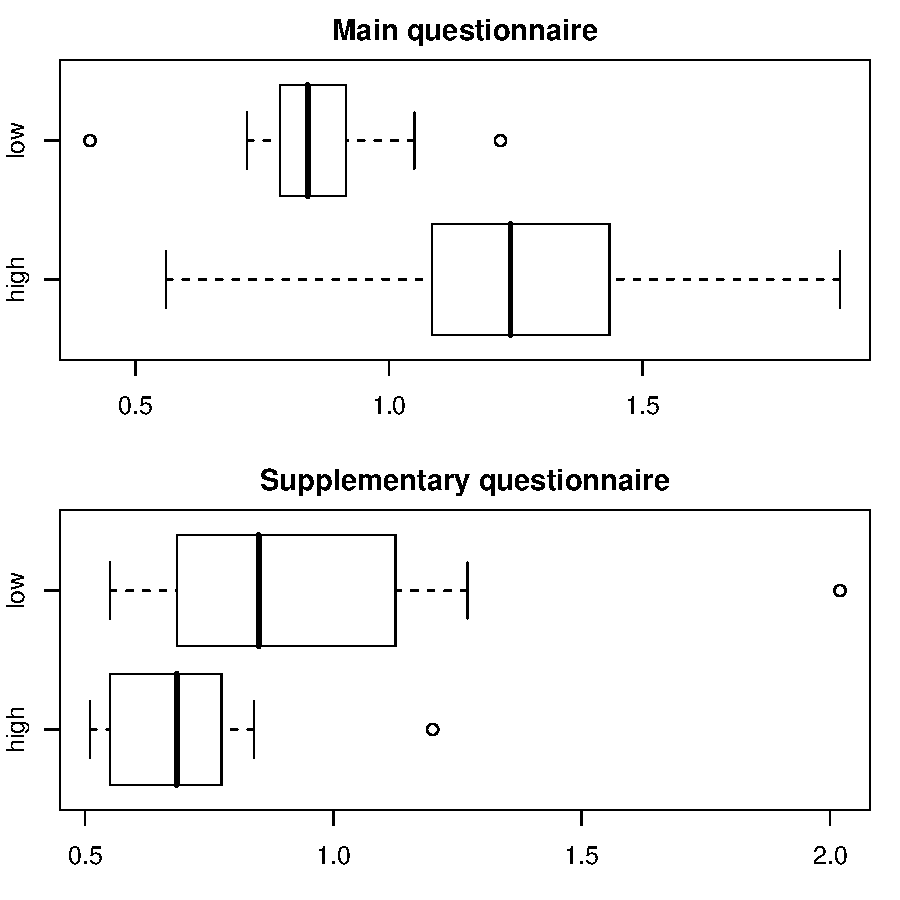
\includegraphics[height=6cm]{../latex/box.pdf} 
\end{frame}

\begin{frame}
\frametitle{A meta-analysis of the categorisation error studies}

\begin{footnotesize}

\begin{tabular}{llrrrr}
\hline
& & & & \multicolumn{2}{c}{95\% C.I}\\
 &  & Estimate & S.E. & lower & upper\\
 \hline
&(Intercept) & 1.04 & 0.36 & 0.31 & 1.77 \\ 
\multicolumn{2}{l}{\textit{Topic}}&  &  &  & \\
 & Doctors & (reference category) &  &  & \\
&Efficacy & 0.06 & 0.10 & -0.14 & 0.27 \\ 
&Job & 0.04 & 0.40 & -0.71 & 0.78 \\ 
&Women & 0.38 & 0.26 & -0.14 & 0.90 \\ 
\multicolumn{2}{l}{\textit{Scale}}&  &  &  & \\ 
 & Direct  & (reference category) &  &  & \\
&Agree-disagree & -0.11 & 0.35 & -0.81 & 0.59 \\ 
&True-false & 0.17 & 0.32 & -0.48 & 0.81 \\ 
\multicolumn{2}{l}{\textit{}   }&  &  &  & \\
\multicolumn{2}{l}{Negative} & -0.50 & 0.23 & -0.96 & -0.02 \\ 
\multicolumn{2}{l}{Main questionnaire} & -0.30 & 0.29 & -0.88 & 0.29 \\ 
\multicolumn{2}{l}{Highest quality} & -0.19 & 0.09 & -0.37 & -0.01 \\ 
\multicolumn{2}{l}{Highest quality $\times$ main} & 0.66 & 0.15 & 0.35 & 0.96 \\ 
\hline
\end{tabular}
Multiple R-Squared: 0.45; Adjusted R-squared: 0.35 

\end{footnotesize}
\end{frame}

\begin{frame}
\frametitle{Conclusions}

	\begin{itemize}[<alert@+>]
				\item Differences in data quality between countries are reduced after the categorisation is taken into account.
				\item Differences in use of the scale seems to play a large role in causing differences between countries.
			\end{itemize}
\end{frame}

\begin{frame}
\frametitle{Recommendations}
	\begin{itemize}[<alert@+>]
				\item One way to prevent categorisation errors is to use continuous or near-continuous scales;
				\item Don't use categories which are difficult to choose in some countries but not in others (e.g. disagree that `Men should take as much responsibility as women for the home and children.' in Slovenia vs. Greece.)
				\item High-quality questions may not be as affected by categorisation errors as low-quality ones!
			\end{itemize}
\end{frame}

\begin{frame}
\frametitle{Further study, problems}
	\begin{itemize}[<alert@+>]
				\item Investigate normality assumption, linearity;
				\item Unobserved heterogeneity;
				\item Prediction of the data quality based on characteristics of the question.
			\end{itemize}
\end{frame}

\begin{frame}
That's it for now. Moltes gr�cies per a la seva atenci�!

	\begin{columns}[T]
		\begin{column}{3cm}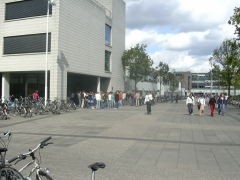
\includegraphics[width=2.55cm]{i/uvt_fac.jpg}\end{column}
		\begin{column}{3cm}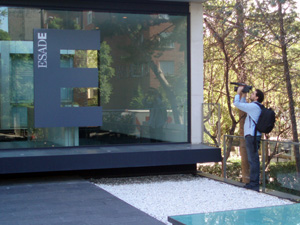
\includegraphics[width=2.5cm]{i/esade_fac.jpg}\end{column}
	\end{columns}		

\end{frame}


\if 1=2

\section{Epilogue: SQP}

\begin{frame}
 \frametitle{The final goal: Survey Quality Predictor (SQP)}

	\begin{enumerate}[<alert@+>]
		\item Estimate the model for all experiments
		\item Save the reliability, validity, and method effect coefficients
		\item Relate the coefficients to different aspects of the question
			\begin{itemize}[<4-|alert@+>]
				\item Complexity of the sentence: no. words/sentence, avg. no. syllables, ...
				\item Response scale: type, no. categories, ...
				\item Formulation of the request: agree-disagree, extra information, ...
				\item Data collection method: computer assisted, interviewer present, ...
			\end{itemize}
		\item Predict the quality of survey questions from their characteristics (SQP)
		\item Improve survey questions
		\item \texttt{http://www.sqp.nl} 
	\end{enumerate}
\end{frame}
\fi

\end{document}
